% Options for packages loaded elsewhere
\PassOptionsToPackage{unicode}{hyperref}
\PassOptionsToPackage{hyphens}{url}
%
\documentclass[
  xelatex,ja=standard, b5paper]{bxjsbook}
\title{がんばらないデータ加工ーRによる繰り返し作業入門ー 前編}
\author{やわらかクジラ}
\date{}

\usepackage{amsmath,amssymb}
\usepackage{lmodern}
\usepackage{iftex}
\ifPDFTeX
  \usepackage[T1]{fontenc}
  \usepackage[utf8]{inputenc}
  \usepackage{textcomp} % provide euro and other symbols
\else % if luatex or xetex
  \usepackage{unicode-math}
  \defaultfontfeatures{Scale=MatchLowercase}
  \defaultfontfeatures[\rmfamily]{Ligatures=TeX,Scale=1}
\fi
% Use upquote if available, for straight quotes in verbatim environments
\IfFileExists{upquote.sty}{\usepackage{upquote}}{}
\IfFileExists{microtype.sty}{% use microtype if available
  \usepackage[]{microtype}
  \UseMicrotypeSet[protrusion]{basicmath} % disable protrusion for tt fonts
}{}
\makeatletter
\@ifundefined{KOMAClassName}{% if non-KOMA class
  \IfFileExists{parskip.sty}{%
    \usepackage{parskip}
  }{% else
    \setlength{\parindent}{0pt}
    \setlength{\parskip}{6pt plus 2pt minus 1pt}}
}{% if KOMA class
  \KOMAoptions{parskip=half}}
\makeatother
\usepackage{xcolor}
\IfFileExists{xurl.sty}{\usepackage{xurl}}{} % add URL line breaks if available
\IfFileExists{bookmark.sty}{\usepackage{bookmark}}{\usepackage{hyperref}}
\hypersetup{
  pdftitle={がんばらないデータ加工ーRによる繰り返し作業入門ー 前編},
  pdfauthor={やわらかクジラ},
  hidelinks,
  pdfcreator={LaTeX via pandoc}}
\urlstyle{same} % disable monospaced font for URLs
\usepackage{color}
\usepackage{fancyvrb}
\newcommand{\VerbBar}{|}
\newcommand{\VERB}{\Verb[commandchars=\\\{\}]}
\DefineVerbatimEnvironment{Highlighting}{Verbatim}{commandchars=\\\{\}}
% Add ',fontsize=\small' for more characters per line
\usepackage{framed}
\definecolor{shadecolor}{RGB}{248,248,248}
\newenvironment{Shaded}{\begin{snugshade}}{\end{snugshade}}
\newcommand{\AlertTok}[1]{\textcolor[rgb]{0.94,0.16,0.16}{#1}}
\newcommand{\AnnotationTok}[1]{\textcolor[rgb]{0.56,0.35,0.01}{\textbf{\textit{#1}}}}
\newcommand{\AttributeTok}[1]{\textcolor[rgb]{0.77,0.63,0.00}{#1}}
\newcommand{\BaseNTok}[1]{\textcolor[rgb]{0.00,0.00,0.81}{#1}}
\newcommand{\BuiltInTok}[1]{#1}
\newcommand{\CharTok}[1]{\textcolor[rgb]{0.31,0.60,0.02}{#1}}
\newcommand{\CommentTok}[1]{\textcolor[rgb]{0.56,0.35,0.01}{\textit{#1}}}
\newcommand{\CommentVarTok}[1]{\textcolor[rgb]{0.56,0.35,0.01}{\textbf{\textit{#1}}}}
\newcommand{\ConstantTok}[1]{\textcolor[rgb]{0.00,0.00,0.00}{#1}}
\newcommand{\ControlFlowTok}[1]{\textcolor[rgb]{0.13,0.29,0.53}{\textbf{#1}}}
\newcommand{\DataTypeTok}[1]{\textcolor[rgb]{0.13,0.29,0.53}{#1}}
\newcommand{\DecValTok}[1]{\textcolor[rgb]{0.00,0.00,0.81}{#1}}
\newcommand{\DocumentationTok}[1]{\textcolor[rgb]{0.56,0.35,0.01}{\textbf{\textit{#1}}}}
\newcommand{\ErrorTok}[1]{\textcolor[rgb]{0.64,0.00,0.00}{\textbf{#1}}}
\newcommand{\ExtensionTok}[1]{#1}
\newcommand{\FloatTok}[1]{\textcolor[rgb]{0.00,0.00,0.81}{#1}}
\newcommand{\FunctionTok}[1]{\textcolor[rgb]{0.00,0.00,0.00}{#1}}
\newcommand{\ImportTok}[1]{#1}
\newcommand{\InformationTok}[1]{\textcolor[rgb]{0.56,0.35,0.01}{\textbf{\textit{#1}}}}
\newcommand{\KeywordTok}[1]{\textcolor[rgb]{0.13,0.29,0.53}{\textbf{#1}}}
\newcommand{\NormalTok}[1]{#1}
\newcommand{\OperatorTok}[1]{\textcolor[rgb]{0.81,0.36,0.00}{\textbf{#1}}}
\newcommand{\OtherTok}[1]{\textcolor[rgb]{0.56,0.35,0.01}{#1}}
\newcommand{\PreprocessorTok}[1]{\textcolor[rgb]{0.56,0.35,0.01}{\textit{#1}}}
\newcommand{\RegionMarkerTok}[1]{#1}
\newcommand{\SpecialCharTok}[1]{\textcolor[rgb]{0.00,0.00,0.00}{#1}}
\newcommand{\SpecialStringTok}[1]{\textcolor[rgb]{0.31,0.60,0.02}{#1}}
\newcommand{\StringTok}[1]{\textcolor[rgb]{0.31,0.60,0.02}{#1}}
\newcommand{\VariableTok}[1]{\textcolor[rgb]{0.00,0.00,0.00}{#1}}
\newcommand{\VerbatimStringTok}[1]{\textcolor[rgb]{0.31,0.60,0.02}{#1}}
\newcommand{\WarningTok}[1]{\textcolor[rgb]{0.56,0.35,0.01}{\textbf{\textit{#1}}}}
\usepackage{longtable,booktabs,array}
\usepackage{calc} % for calculating minipage widths
% Correct order of tables after \paragraph or \subparagraph
\usepackage{etoolbox}
\makeatletter
\patchcmd\longtable{\par}{\if@noskipsec\mbox{}\fi\par}{}{}
\makeatother
% Allow footnotes in longtable head/foot
\IfFileExists{footnotehyper.sty}{\usepackage{footnotehyper}}{\usepackage{footnote}}
\makesavenoteenv{longtable}
\usepackage{graphicx}
\makeatletter
\def\maxwidth{\ifdim\Gin@nat@width>\linewidth\linewidth\else\Gin@nat@width\fi}
\def\maxheight{\ifdim\Gin@nat@height>\textheight\textheight\else\Gin@nat@height\fi}
\makeatother
% Scale images if necessary, so that they will not overflow the page
% margins by default, and it is still possible to overwrite the defaults
% using explicit options in \includegraphics[width, height, ...]{}
\setkeys{Gin}{width=\maxwidth,height=\maxheight,keepaspectratio}
% Set default figure placement to htbp
\makeatletter
\def\fps@figure{htbp}
\makeatother
\setlength{\emergencystretch}{3em} % prevent overfull lines
\providecommand{\tightlist}{%
  \setlength{\itemsep}{0pt}\setlength{\parskip}{0pt}}
\setcounter{secnumdepth}{5}
\makeatletter
\def\emptypage@emptypage{%
    \hbox{}%
    \thispagestyle{headings}%
    \newpage%    
}%
\def\cleardoublepage{%
        \clearpage%
        \if@twoside%
            \ifodd\c@page%
                % do nothing
            \else%
                \emptypage@emptypage%
            \fi%
        \fi%
    }%
\makeatother
\ifLuaTeX
  \usepackage{selnolig}  % disable illegal ligatures
\fi

\begin{document}
\maketitle

{
\setcounter{tocdepth}{1}
\tableofcontents
}
\hypertarget{hajimeni}{%
\chapter*{はじめに}\label{hajimeni}}
\addcontentsline{toc}{chapter}{はじめに}

\begin{itemize}
\tightlist
\item
  本書の目的

  \begin{itemize}
  \tightlist
  \item
    データ加工での面倒な作業をRでらくらく実行できるようになるための基礎知識を紹介
  \end{itemize}
\item
  本書の内容

  \begin{itemize}
  \tightlist
  \item
    実際は核心の部分に入る前の準備段階までにとどまる。タイトルに「前編」とあるのはその理由による
  \item
    本当は,複数データセットの複数変数をいっぺんに加工,集計,視覚化!みたいなのをまとめたかったが,そこに入るための事前知識が思っていたより多かったため,まずはそれらを解説することに徹した
  \item
    既刊書では省いたRのモダンな方法を使ったデータ加工の過程(例:前処理、データクリーニング、データクレンジング、データラングリングなど)で用いる基本関数の紹介
  \end{itemize}
\item
  執筆動機

  \begin{itemize}
  \tightlist
  \item
    本書を書こうと思ったのは拙既刊書\href{https://techbookfest.org/product/4794168259903488?productVariantID=5913872206659584}{『Rで読むExcelファイル』}と同じく,「RとRStudioを使いたい!と思う人がもっと増えればいいのに」という願いから
  \end{itemize}
\item
  今後の展望

  \begin{itemize}
  \tightlist
  \item
    よりタイトルの内容に沿った次回作の「後編」(もしかしたら「中編」も)をお楽しみに!
  \end{itemize}
\end{itemize}

\hypertarget{ux672cux66f8ux306eux7279ux5fb4}{%
\section*{本書の特徴}\label{ux672cux66f8ux306eux7279ux5fb4}}
\addcontentsline{toc}{section}{本書の特徴}

\begin{itemize}
\tightlist
\item
  タイトルの「がんばらない」とは,\textbf{単純作業のくり返しに無駄なエネルギーを注がなくてよいように}すること
\item
  扱う内容は自分が学び始めの時に教えてもらいたかったこと
\item
  これまでの解説で不足していると考えられるポイント

  \begin{itemize}
  \tightlist
  \item
    便利な関数や基本的な使い方の解説は多いが,データ加工の実務上知りたいコード例が豊富なわけではない
  \item
    \textbf{同じ作業を大量の変数についてくり返し実行}したい時のやり方の解説は少ない
  \end{itemize}
\item
  本書の強み

  \begin{itemize}
  \tightlist
  \item
    くり返し同じ作業する部分を効率化したコードを併せて解説する点
  \item
    自分の学習経験から,そのコード例が知りたかったんだ!という実用的な方法を整理
  \end{itemize}
\item
  まずモダンなRのデータ加工法での基本の書き方を解説した後に,\textbf{【効率化】}でより効率的にコードを書く解説を行う
\item
  \textbf{【効率化】}のタグが本書の核心になる。手作業の繰り返しをなるべく避けることが目指すべき点
\item
  冗長だが【別解】を示すことで様々な関数の働きを理解でき,手持ちの武器が増えデータ加工の幅が広がる
\end{itemize}

\hypertarget{ux60f3ux5b9aux8aadux8005}{%
\subsection*{想定読者}\label{ux60f3ux5b9aux8aadux8005}}
\addcontentsline{toc}{subsection}{想定読者}

\begin{itemize}
\tightlist
\item
  RとRStudioをダウンロードしてPCにインストールまでできることが最低条件

  \begin{itemize}
  \tightlist
  \item
    web上に様々な解説があり,あとは基本的にOKしていけばできるはず
  \end{itemize}
\item
  初学者から始めてちょっと背伸びできるくらいまでが到達目標
\end{itemize}

\hypertarget{ux5404ux30bbux30afux30b7ux30e7ux30f3ux306eux6982ux8981}{%
\subsection*{各セクションの概要}\label{ux5404ux30bbux30afux30b7ux30e7ux30f3ux306eux6982ux8981}}
\addcontentsline{toc}{subsection}{各セクションの概要}

まず\ref{premise}章では、RとRStudioに初めて触れる方,初学者を対象とした前提知識を解説する。ゆくゆく楽をするためには避けて通れない知識なので,用語になじんでおきたい

\ref{select}章はデータの列(変数)を選ぶ方法を解説する。データをコンパクトにしたり,後のデータ解析等で必要な変数を取得したりするなど,データ加工プロセス全体で必要な基本知識もあるので最初に学んでおきたい

\ref{rename}章はデータの列名(変数名)を変える方法について解説する。単純に見えるがデータ加工の際になくてはならない技術である。効率化させるためには初心者から少し脱する必要があり,奥が深い

\ref{filter}章はデータの行(ケースまたはオブザベーション)を選ぶ方法を解説する。データや加工した結果,分析した結果をコンパクトにするのに役立つ。

\ref{mutate}章はデータに新しい列を追加する方法について解説する。例えば合計点の作成や,年齢層カテゴリや2区分変数(いわゆるダミー変数)の作成など,変数を計算して新しい変数を作る作業はよく発生する。効率化のために避けて通れない\texttt{across(\ )}についてもここで解説する

\ref{summarise}章は要約値の計算について解説する。実務では大量の変数を一気に処理する必要がある場面が多いので,効率化を意識した説明を多く入れている

\hypertarget{ux57f7ux7b46ux74b0ux5883}{%
\subsection*{執筆環境}\label{ux57f7ux7b46ux74b0ux5883}}
\addcontentsline{toc}{subsection}{執筆環境}

\begin{itemize}
\tightlist
\item
  本書は\href{https://bookdown.org/}{bookdown}にて執筆
\end{itemize}

\hypertarget{rux304aux3088ux3073rstudioux30d1ux30c3ux30b1ux30fcux30b8ux306eux30d0ux30fcux30b8ux30e7ux30f3}{%
\subsubsection*{RおよびRStudio、パッケージのバージョン}\label{rux304aux3088ux3073rstudioux30d1ux30c3ux30b1ux30fcux30b8ux306eux30d0ux30fcux30b8ux30e7ux30f3}}
\addcontentsline{toc}{subsubsection}{RおよびRStudio、パッケージのバージョン}

\begin{itemize}
\tightlist
\item
  rstudioだけなぜか表示されないので手動で\ldots{}

  \begin{itemize}
  \tightlist
  \item
    バージョン 2021.09.1+372 Ghost Orchid (desktop)
  \end{itemize}
\end{itemize}

\begin{tabular}{l|l}
\hline
ind & values\\
\hline
version & R version 4.1.0 (2021-05-18)\\
\hline
os & Windows 10 x64 (build 19043)\\
\hline
system & x86\_64, mingw32\\
\hline
date & 2022-01-16\\
\hline
\end{tabular}

\begin{tabular}{l|l}
\hline
package & loadedversion\\
\hline
bookdown & 0.24\\
\hline
tidyverse & 1.3.1\\
\hline
\end{tabular}

\hypertarget{ux6ce8ux610fux4e8bux9805ux306aux3069}{%
\section*{注意事項など}\label{ux6ce8ux610fux4e8bux9805ux306aux3069}}
\addcontentsline{toc}{section}{注意事項など}

\begin{itemize}
\tightlist
\item
  本書の内容はすべてwindows環境を想定
\item
  この本に書いてある内容は、筆者が学習したことをまとめているものにすぎないため、正常な動作の保証はできない。使用する際は、自己責任で
\end{itemize}

\hypertarget{ux30e9ux30a4ux30bbux30f3ux30b9}{%
\section*{ライセンス}\label{ux30e9ux30a4ux30bbux30f3ux30b9}}
\addcontentsline{toc}{section}{ライセンス}

\begin{itemize}
\tightlist
\item
  \href{https://creativecommons.org/licenses/by-sa/4.0/}{CC BY-SA 4.0}

  \begin{itemize}
  \tightlist
  \item
    引用例:やわらかクジラ(2021)『がんばらないデータ加工ーRによる繰り返し作業入門ー 前編』. (サークル名:ヤサイゼリー), 技術書展12にて頒布
  \item
    ただし,ライセンスの適用は本書での著作部分のみとなり,用いているデータやパッケージや画像などはそれぞれのライセンスに準じる
  \end{itemize}
\item
  本書の内容は、\href{https://github.com/izunyan/gisho12}{githubレポジトリ}ですべて公開
\end{itemize}

\hypertarget{association}{%
\section*{関連情報}\label{association}}
\addcontentsline{toc}{section}{関連情報}

\begin{itemize}
\tightlist
\item
  \href{https://techbookfest.org/product/4794168259903488?productVariantID=5913872206659584}{『Rで読むExcelファイル』}

  \begin{itemize}
  \tightlist
  \item
    技術書典9で頒布したRでのExcelおよびcsvファイル読み込み解説本
  \item
    \href{https://izunyan.github.io/excel_r/}{github}
  \end{itemize}
\item
  \href{https://izunyan.github.io/practice_ggplot2/}{ggplot2の辞書}

  \begin{itemize}
  \tightlist
  \item
    視覚化のための\texttt{ggplot2}パッケージの辞書的メモ
  \end{itemize}
\end{itemize}

\hypertarget{premise}{%
\chapter{前提知識}\label{premise}}

\begin{itemize}
\tightlist
\item
  ここに出てくる用語は初学者にとってなじみがないものばかりかもしれないが,Rでデータ加工をらくらくできるようになるためには避けて通れない
\end{itemize}

\hypertarget{p-howtoread}{%
\section{本書に出てくるコード部分の見方}\label{p-howtoread}}

\begin{itemize}
\tightlist
\item
  グレーの背景部分はRのコードが書いてあり,その下の\texttt{\#\#}で始まる部分は出力結果を表す
\end{itemize}

\begin{Shaded}
\begin{Highlighting}[]
\DecValTok{1} \SpecialCharTok{+} \DecValTok{1}
\end{Highlighting}
\end{Shaded}

\begin{verbatim}
## [1] 2
\end{verbatim}

\begin{itemize}
\tightlist
\item
  ここでは\texttt{1\ +\ 1}がコード部分で,\texttt{\#\#\ {[}1{]}\ 2}が出力結果部分
\item
  \texttt{{[}1{]}}というのは,その次にくる値(ここでは1つしかないが)が何番目にあるかを示している
\item
  たとえば,1から50までの数値を出力してみる

  \begin{itemize}
  \tightlist
  \item
    コロン\texttt{:}で最初と最後の値をつなぐことで連番を表現できる
  \end{itemize}
\end{itemize}

\begin{Shaded}
\begin{Highlighting}[]
\DecValTok{1}\SpecialCharTok{:}\DecValTok{50}
\end{Highlighting}
\end{Shaded}

\begin{verbatim}
##  [1]  1  2  3  4  5  6  7  8  9 10 11 12 13 14 15 16 17 18 19 20 21 22 23 24 25
## [26] 26 27 28 29 30 31 32 33 34 35 36 37 38 39 40 41 42 43 44 45 46 47 48 49 50
\end{verbatim}

\begin{itemize}
\tightlist
\item
  コード部分に\texttt{\#}で始まる文章がある場合は,コメントを表す。ここは実行されないので説明のために書かれる
\end{itemize}

\begin{Shaded}
\begin{Highlighting}[]
\CommentTok{\# *(アスタリスク) は掛け算であることを示す}

\DecValTok{2} \SpecialCharTok{*} \DecValTok{3}  \CommentTok{\# ここにもコメントを入れられる}
\end{Highlighting}
\end{Shaded}

\begin{verbatim}
## [1] 6
\end{verbatim}

\hypertarget{p-project}{%
\section{プロジェクト}\label{p-project}}

\begin{itemize}
\tightlist
\item
  データを加工して解析する際に、1つのフォルダ(サブフォルダも含む)の中に関連するデータやコードなどをまとめておき、そのフォルダを\textbf{プロジェクト}と設定する

  \begin{itemize}
  \tightlist
  \item
    これにより、ファイルの読み書きの際の場所指定をいちいち意識しないで作業できるようになる
  \end{itemize}
\item
  RStudio画面の右上にProject設定のメニューがある

  \begin{itemize}
  \tightlist
  \item
    \texttt{Project\ (None)\ \textgreater{}\ New\ Project\ \textgreater{}\ Existing\ Directory}と選び,プロジェクトにしたいフォルダを設定する(Figure\ref{fig:project})
  \end{itemize}
\end{itemize}

\begin{figure}

{\centering 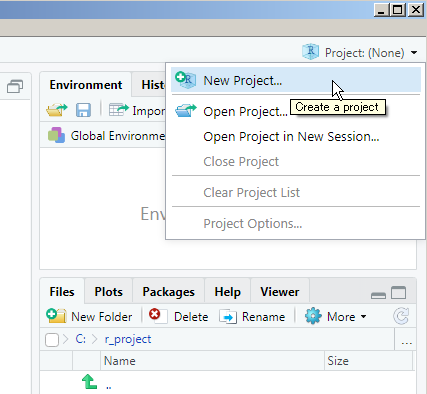
\includegraphics[width=7.11in]{images/project} 

}

\caption{プロジェクトの設定}\label{fig:project}
\end{figure}

\hypertarget{p-package}{%
\section{パッケージ}\label{p-package}}

\begin{itemize}
\tightlist
\item
  様々な関数やデータなどがまとまっていて,読み込むと色々なことができる

  \begin{itemize}
  \tightlist
  \item
    逆にいえば読み込まないと便利な作業ができないことが多い
  \end{itemize}
\item
  インストールされているパッケージはRStudioのデフォルト画面で右下にあるウィンドウ(ペインと呼ぶ)のパッケージタブで確認可能(Figure\ref{fig:pinst})\\
\item
  入っていないパッケージは,インターネットにつながっていれば以下の方法でインストールできる

  \begin{itemize}
  \tightlist
  \item
    パッケージタブの\texttt{install}をクリックして出てくるウィンドウでパッケージ名を入力
  \item
    コマンドから\texttt{install.packages("パッケージ名をここに入れる")}
  \end{itemize}
\end{itemize}

\begin{figure}

{\centering 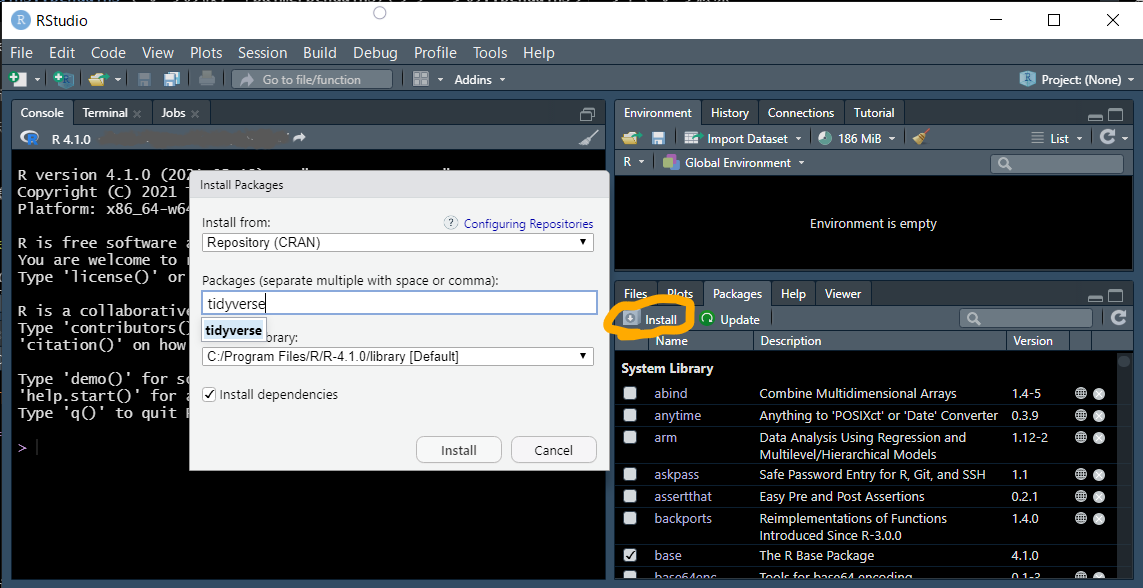
\includegraphics[width=0.6\linewidth]{images/package_install} 

}

\caption{パッケージタブからのインストール}\label{fig:pinst}
\end{figure}

\begin{itemize}
\tightlist
\item
  例:\texttt{library(tidyverse)}または\texttt{require(tidyverse)} のように書くことで読み込める
\item
  パッケージを読み込まなくても,\texttt{パッケージ名::関数名(\ )}でパッケージ内の関数が使える

  \begin{itemize}
  \tightlist
  \item
    どのパッケージの関数か明示するのにも便利なので,本書では多用する
  \item
    以下,例えば「パッケージ\texttt{dplyr}の関数\texttt{select(\ )}」は\texttt{dplyr::select(\ )}と表現する
  \end{itemize}
\end{itemize}

\hypertarget{p-function}{%
\section{関数}\label{p-function}}

\begin{itemize}
\tightlist
\item
  適切な値や変数などを指定すれば,データの処理や計算,統計解析など様々な処理を簡単に実行してくれる

  \begin{itemize}
  \tightlist
  \item
    データ加工の技術は,色々な便利関数をどの場面でどうやって使うかにつきる
  \end{itemize}
\item
  例えば\texttt{mean(\ )}などのように\texttt{関数名(\ )}で出てくるので,\texttt{(\ )}で囲まれてる所を見たらほぼ関数だと思えばよさそう
\item
  \texttt{(\ )}の中に入る値を\textbf{引数}(ひきすう)と呼ぶ
\item
  引数は\texttt{,}でつないで追加していき,これによって実行したい処理のカスタマイズが可能

  \begin{itemize}
  \tightlist
  \item
    関数の\texttt{(\ )}の最初の位置に来るものを\textbf{第一引数}という
  \end{itemize}
\end{itemize}

\hypertarget{p-function-ex}{%
\subsection{例}\label{p-function-ex}}

\hypertarget{p-function-ex-c}{%
\subsubsection{複数のものを1つにする: c( )}\label{p-function-ex-c}}

\begin{itemize}
\tightlist
\item
  \textbf{ベクトル}を作る(複数のものを1つにする)ための関数

  \begin{itemize}
  \tightlist
  \item
    ベクトルと聞くと数学苦手だった人はいやな記憶を思い出すかもしれないが,Rではとにかく「\textbf{複数のものを1つにしたもの}」と理解しておけば何となると思う
  \end{itemize}
\item
  \texttt{c()}は慣れてる人は当たり前に使っているので,初学者にとって理解しとくとよい最重要関数と思われる
\item
  ベクトルは,後に解説するデータフレームでの列単位のデータを扱う際にも有用
\end{itemize}

\begin{Shaded}
\begin{Highlighting}[]
\FunctionTok{c}\NormalTok{(}\DecValTok{1}\NormalTok{,}\DecValTok{2}\NormalTok{,}\DecValTok{3}\NormalTok{)}
\end{Highlighting}
\end{Shaded}

\begin{verbatim}
## [1] 1 2 3
\end{verbatim}

\begin{Shaded}
\begin{Highlighting}[]
\FunctionTok{c}\NormalTok{(}\StringTok{"a"}\NormalTok{, }\StringTok{"b"}\NormalTok{, }\StringTok{"c"}\NormalTok{) }\CommentTok{\# " "で囲まれる値は文字を表す}
\end{Highlighting}
\end{Shaded}

\begin{verbatim}
## [1] "a" "b" "c"
\end{verbatim}

\begin{Shaded}
\begin{Highlighting}[]
\CommentTok{\# 複数あるように見えるが実は1つのベクトルになっている例}
\DecValTok{1}\SpecialCharTok{:}\DecValTok{10}
\end{Highlighting}
\end{Shaded}

\begin{verbatim}
##  [1]  1  2  3  4  5  6  7  8  9 10
\end{verbatim}

\hypertarget{p-function-ex-m}{%
\subsubsection{平均値:mean( )}\label{p-function-ex-m}}

\begin{itemize}
\tightlist
\item
  引数にベクトルを入れることで平均値を計算する
\end{itemize}

\begin{Shaded}
\begin{Highlighting}[]
\FunctionTok{mean}\NormalTok{(}\FunctionTok{c}\NormalTok{(}\DecValTok{1}\NormalTok{,}\DecValTok{2}\NormalTok{,}\DecValTok{3}\NormalTok{))}
\end{Highlighting}
\end{Shaded}

\begin{verbatim}
## [1] 2
\end{verbatim}

\begin{Shaded}
\begin{Highlighting}[]
\CommentTok{\# 欠損値(NA)があると結果がNA}
\FunctionTok{mean}\NormalTok{(}\FunctionTok{c}\NormalTok{(}\DecValTok{1}\NormalTok{, }\ConstantTok{NA}\NormalTok{, }\DecValTok{3}\NormalTok{))}
\end{Highlighting}
\end{Shaded}

\begin{verbatim}
## [1] NA
\end{verbatim}

\begin{Shaded}
\begin{Highlighting}[]
\CommentTok{\# 引数にna.rm = TRUEを追加すると結果が出る}
\CommentTok{\# 基本的に実務上は常につけておいたほうがよい}
\FunctionTok{mean}\NormalTok{(}\FunctionTok{c}\NormalTok{(}\DecValTok{1}\NormalTok{, }\ConstantTok{NA}\NormalTok{, }\DecValTok{3}\NormalTok{), }\AttributeTok{na.rm =} \ConstantTok{TRUE}\NormalTok{)}
\end{Highlighting}
\end{Shaded}

\begin{verbatim}
## [1] 2
\end{verbatim}

\hypertarget{p-object}{%
\section{オブジェクト}\label{p-object}}

\begin{itemize}
\tightlist
\item
  計算の結果や,複数の数値や文字など(他にも色々)を1つの文字列に格納することができ,その後のコードで活用できる
\item
  \texttt{\textless{}-}の矢印の先にあるのがオブジェクト。RStudioではショートカット\texttt{alt\ +\ -}で出せる(Macは\texttt{Option\ +\ -})
\item
  この後説明するデータフレームもオブジェクトに入れられる

  \begin{itemize}
  \tightlist
  \item
    データの少ないミニデータを作る時や,計算結果を格納するときに多用
  \end{itemize}
\end{itemize}

\hypertarget{p-object-ex}{%
\subsection{例}\label{p-object-ex}}

\begin{Shaded}
\begin{Highlighting}[]
\NormalTok{res }\OtherTok{\textless{}{-}} \DecValTok{1} \SpecialCharTok{+} \DecValTok{1}
\NormalTok{res}
\end{Highlighting}
\end{Shaded}

\begin{verbatim}
## [1] 2
\end{verbatim}

\begin{Shaded}
\begin{Highlighting}[]
\NormalTok{res2 }\OtherTok{\textless{}{-}} \FunctionTok{c}\NormalTok{(}\DecValTok{1}\NormalTok{, }\DecValTok{2}\SpecialCharTok{:}\DecValTok{4}\NormalTok{, }\DecValTok{5}\NormalTok{)}
\NormalTok{res2}
\end{Highlighting}
\end{Shaded}

\begin{verbatim}
## [1] 1 2 3 4 5
\end{verbatim}

\begin{Shaded}
\begin{Highlighting}[]
\NormalTok{res3 }\OtherTok{\textless{}{-}} \FunctionTok{c}\NormalTok{(}\StringTok{"a"}\NormalTok{, }\StringTok{"b"}\NormalTok{)}
\NormalTok{res3}
\end{Highlighting}
\end{Shaded}

\begin{verbatim}
## [1] "a" "b"
\end{verbatim}

\begin{Shaded}
\begin{Highlighting}[]
\FunctionTok{rm}\NormalTok{(res, res2, res3)}
\end{Highlighting}
\end{Shaded}

\hypertarget{p-df}{%
\section{データフレーム}\label{p-df}}

\begin{itemize}
\tightlist
\item
  行(ケースまたはオブザベーション)と列(変数)が碁盤の目のようになった集まりの形のデータ(Figure\ref{fig:dfr})

  \begin{itemize}
  \tightlist
  \item
    Excelで表現するのであれば通常1行目に列名が入り、2行目以降が個別のケース(データ)を表す形。Rのデータフレームでは列名は別途与えられ,1行目からケースが表される(Figure\ref{fig:dfxl})
  \item
    データ解析において便利で分かりやすいため、本書ではデータフレームの形で説明していく
  \item
    Rのモダンな方法では,データの加工や統計処理のプロセスをデータフレームの形で返すことが多い
  \item
    上記のような状態を\textbf{tidy}(読み:タイディー,意味:整然)と呼び,データ加工において理想的な形とされている
  \end{itemize}
\end{itemize}

\begin{figure}

{\centering 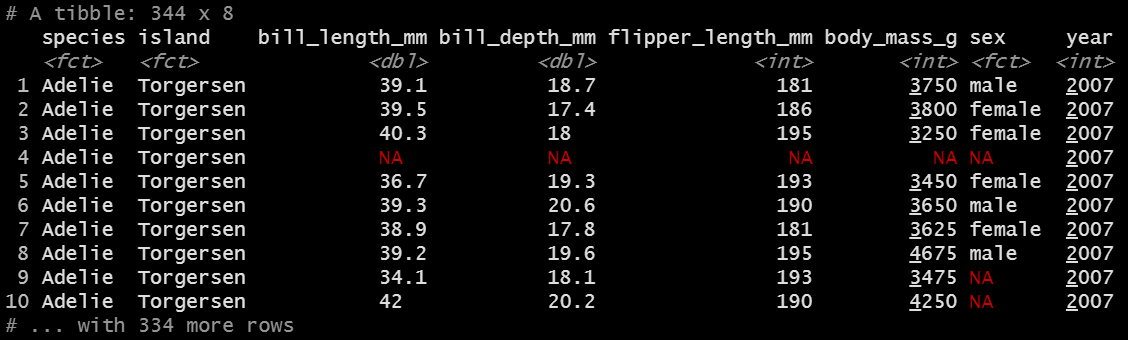
\includegraphics[width=0.6\linewidth]{images/dfr} 

}

\caption{Rのデータフレーム(tibble形式)}\label{fig:dfr}
\end{figure}

\begin{figure}

{\centering 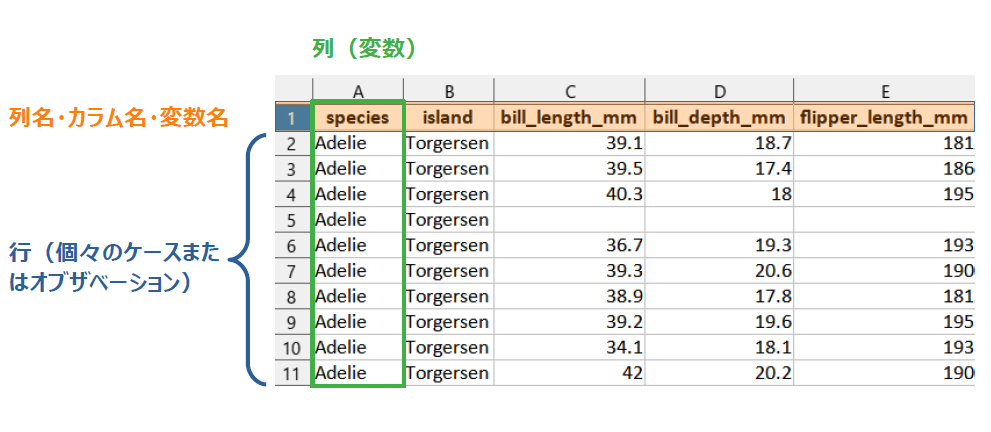
\includegraphics[width=0.6\linewidth]{images/df_xl} 

}

\caption{Excel画面風なイメージ}\label{fig:dfxl}
\end{figure}

\begin{itemize}
\tightlist
\item
  オブジェクトに格納することで,別のデータフレームを作れる
\item
  列単位で取り出すとベクトルになる
\item
  本書では,データフレームの中でも表示に便利なtibble形式を使う
\item
  本書では紙面の都合上,表示行数をしぼっているが,任意の行数を見たいときは\texttt{print(\ )}関数で出力ごとに設定
\end{itemize}

\hypertarget{p-df-main}{%
\subsection{本書で使う主なデータ}\label{p-df-main}}

\hypertarget{p-df-main-p}{%
\subsubsection{ペンギンデータ}\label{p-df-main-p}}


\includegraphics{images/penguins_logo.png}

\begin{itemize}
\tightlist
\item
  \texttt{palmerpenguins}パッケージのpenguinsデータ(CC0)
\end{itemize}

\begin{Shaded}
\begin{Highlighting}[]
\CommentTok{\# パッケージが入ってなければ下記実行}
\CommentTok{\# install.packages("palmerpenguins")}

\NormalTok{palmerpenguins}\SpecialCharTok{::}\NormalTok{penguins}
\end{Highlighting}
\end{Shaded}

\begin{verbatim}
## # A tibble: 344 x 8
##   species island    bill_length_mm bill_depth_mm flipper_length_~
##   <fct>   <fct>              <dbl>         <dbl>            <int>
## 1 Adelie  Torgersen           39.1          18.7              181
## 2 Adelie  Torgersen           39.5          17.4              186
## 3 Adelie  Torgersen           40.3          18                195
## # ... with 341 more rows, and 3 more variables:
## #   body_mass_g <int>, sex <fct>, year <int>
\end{verbatim}

\begin{itemize}
\tightlist
\item
  tibble形式のデータフレームの出力の見方

  \begin{itemize}
  \tightlist
  \item
    出力の最上段にある\texttt{A\ tibble:\ 344\ x\ 8}で,tibble形式のデータフレーム,344行 × 8列という情報が分かる
  \item
    flipper\_length\_\textsubscript{のように,長い変数名は}で省略して表示される
  \item
    変数名の下の行にある\texttt{\textless{}fct\textgreater{}}, \texttt{\textless{}dbl\textgreater{}}, \texttt{\textless{}int\textgreater{}}は変数の型を示し,それぞれ因子型,数値型,整数型であることを示している。詳しくは\ref{mu-kata}で説明する
  \item
    下から2行目にある\texttt{...\ with\ 341\ more\ rows,\ and\ 3\ more\ variables:}で,さらに341行と3列が非表示であることが分かる
  \item
    非表示になった変数名は最下部に表示される
  \end{itemize}
\item
  tibble型のデフォルトは最初の10行のみ表示され,本書では最初の3行のみに絞っているが,10行を越えて表示させたい場合は,\texttt{print(\ )}関数を使う
\end{itemize}

\begin{Shaded}
\begin{Highlighting}[]
\NormalTok{palmerpenguins}\SpecialCharTok{::}\NormalTok{penguins }\SpecialCharTok{\%\textgreater{}\%} 
  \FunctionTok{print}\NormalTok{(}\AttributeTok{n =} \DecValTok{15}\NormalTok{)}
\end{Highlighting}
\end{Shaded}

\begin{verbatim}
## # A tibble: 344 x 8
##    species island   bill_length_mm bill_depth_mm flipper_length_~
##    <fct>   <fct>             <dbl>         <dbl>            <int>
##  1 Adelie  Torgers~           39.1          18.7              181
##  2 Adelie  Torgers~           39.5          17.4              186
##  3 Adelie  Torgers~           40.3          18                195
##  4 Adelie  Torgers~           NA            NA                 NA
##  5 Adelie  Torgers~           36.7          19.3              193
##  6 Adelie  Torgers~           39.3          20.6              190
##  7 Adelie  Torgers~           38.9          17.8              181
##  8 Adelie  Torgers~           39.2          19.6              195
##  9 Adelie  Torgers~           34.1          18.1              193
## 10 Adelie  Torgers~           42            20.2              190
## 11 Adelie  Torgers~           37.8          17.1              186
## 12 Adelie  Torgers~           37.8          17.3              180
## 13 Adelie  Torgers~           41.1          17.6              182
## 14 Adelie  Torgers~           38.6          21.2              191
## 15 Adelie  Torgers~           34.6          21.1              198
## # ... with 329 more rows, and 3 more variables:
## #   body_mass_g <int>, sex <fct>, year <int>
\end{verbatim}

\hypertarget{p-pipe}{%
\section{\%\textgreater\% (パイプ演算子)}\label{p-pipe}}

\begin{itemize}
\tightlist
\item
  名前は\textbf{パイプ}で発音は''\emph{and then}'' (\href{https://adv-r.hadley.nz/functions.html\#function-composition}{参照})
\item
  コードを読みやすくするための便利な機能を持つ演算子。初めてみた人は全然わからないと思うが,この本を読んでコードを書きはじめてみたらこれなしではいられなくなるくらいお世話になると思う

  \begin{itemize}
  \tightlist
  \item
    主に使用が想定される場面でざっくりいうと,「このデータフレームに対して\texttt{\%\textgreater{}\%}の後にある関数を適用する」という機能
  \item
    具体的な使用法は\ref{select-standard-pipe}で解説
  \end{itemize}
\item
  RStudioのショートカットは\texttt{Ctrl\ +\ Shift\ +\ M}(Macは\texttt{Cmd\ +\ Shift\ +\ M})。たぶん,RStudio以外でもこのショートカット押してしまうぐらい中毒性がある
\item
  R version 4.1からは\texttt{\textbar{}\textgreater{}}が大体同じ機能を持つ演算子して実装されたので,特にパッケージの読み込みをせずに使えるようになった。こちらを使う説明も今後増えていくと思われる

  \begin{itemize}
  \tightlist
  \item
    ショートカットで出るパイプを\texttt{\textbar{}\textgreater{}}に切り替えたい場合は,RStudioの\texttt{Tools\ \textgreater{}\ Global\ Options\ \textgreater{}\ Code\ \textgreater{}\ Editing\ \textgreater{}\ use\ native\ pipe\ operator}にチェックを入れる
  \item
    現時点ではデータフレームを第一引数へ渡す形式でない関数の場合(回帰分析の\texttt{lm(\ )}など),工夫が必要な場合があるようなので,本書では\texttt{\%\textgreater{}\%}を使用
  \end{itemize}
\end{itemize}

\hypertarget{select}{%
\chapter{列(変数)を選ぶ:select}\label{select}}

\begin{itemize}
\tightlist
\item
  \texttt{dplyr:select(\ )}
\item
  tidyな世界では「列名 = 変数名」
\item
  変数が多い時に関心ある変数に限定したデータにしたい
\item
  関心ある変数の名前を取得したい
\item
  後々出てくる繰り返し作業で便利なヘルパー関数
\end{itemize}

\hypertarget{select-read}{%
\section{データ読み込み}\label{select-read}}

\begin{itemize}
\tightlist
\item
  データの指定を簡単にするために,penguinsデータを\texttt{df}と読み込む
\item
  \texttt{palmerpenguins::penguins}というのは,「palmerpenguinsパッケージの::penguinsデータ」という意味
\end{itemize}

\begin{Shaded}
\begin{Highlighting}[]
\FunctionTok{library}\NormalTok{(tidyverse)}

\NormalTok{df }\OtherTok{\textless{}{-}} 
\NormalTok{  palmerpenguins}\SpecialCharTok{::}\NormalTok{penguins}

\CommentTok{\# データの表示  }
\NormalTok{df }
\end{Highlighting}
\end{Shaded}

\begin{verbatim}
## # A tibble: 344 x 8
##   species island    bill_length_mm bill_depth_mm flipper_length_~
##   <fct>   <fct>              <dbl>         <dbl>            <int>
## 1 Adelie  Torgersen           39.1          18.7              181
## 2 Adelie  Torgersen           39.5          17.4              186
## 3 Adelie  Torgersen           40.3          18                195
## # ... with 341 more rows, and 3 more variables:
## #   body_mass_g <int>, sex <fct>, year <int>
\end{verbatim}

\begin{itemize}
\tightlist
\item
  読み込みの様々な方法については拙書\href{https://izunyan.github.io/excel_r/}{『Rで読むExcelファイル』}参照
\end{itemize}

\hypertarget{select-standard}{%
\section{基本}\label{select-standard}}

\begin{itemize}
\tightlist
\item
  \texttt{select(\ )}の中に関心のある変数名を\texttt{,}をつけて並べる

  \begin{itemize}
  \tightlist
  \item
    変数は1つからOK
  \end{itemize}
\end{itemize}

\begin{Shaded}
\begin{Highlighting}[]
\NormalTok{df }\SpecialCharTok{\%\textgreater{}\%} 
  \FunctionTok{select}\NormalTok{(bill\_length\_mm, bill\_depth\_mm)}
\end{Highlighting}
\end{Shaded}

\begin{verbatim}
## # A tibble: 344 x 2
##   bill_length_mm bill_depth_mm
##            <dbl>         <dbl>
## 1           39.1          18.7
## 2           39.5          17.4
## 3           40.3          18  
## # ... with 341 more rows
\end{verbatim}

\begin{itemize}
\tightlist
\item
  新しいデータフレームを作りたい場合は\texttt{\textless{}-}を使って新しいオブジェクトに格納する
\end{itemize}

\begin{Shaded}
\begin{Highlighting}[]
\NormalTok{df2 }\OtherTok{\textless{}{-}} 
\NormalTok{  df }\SpecialCharTok{\%\textgreater{}\%} \FunctionTok{select}\NormalTok{(bill\_length\_mm)}

\NormalTok{df2}
\end{Highlighting}
\end{Shaded}

\begin{verbatim}
## # A tibble: 344 x 1
##   bill_length_mm
##            <dbl>
## 1           39.1
## 2           39.5
## 3           40.3
## # ... with 341 more rows
\end{verbatim}

\begin{Shaded}
\begin{Highlighting}[]
\FunctionTok{rm}\NormalTok{(df2)}
\end{Highlighting}
\end{Shaded}

\hypertarget{select-standard-pipe}{%
\subsection{【補足】\%\textgreater\% の意味}\label{select-standard-pipe}}

\begin{itemize}
\tightlist
\item
  \ref{p-pipe}で説明したパイプ演算子の実例を解説する
\item
  基本的に\texttt{select(\ )}を始めとしたモダンなRの処理は,以下のように第一引数にデータフレームを指定する
\end{itemize}

\begin{Shaded}
\begin{Highlighting}[]
\FunctionTok{select}\NormalTok{(df, bill\_length\_mm)}
\end{Highlighting}
\end{Shaded}

\begin{verbatim}
## # A tibble: 344 x 1
##   bill_length_mm
##            <dbl>
## 1           39.1
## 2           39.5
## 3           40.3
## # ... with 341 more rows
\end{verbatim}

\begin{itemize}
\tightlist
\item
  \texttt{\%\textgreater{}\%}の役割は,その左側にあるものを右側の関数の第一引数に入れる,ということなので,第一引数にデータフレームが来ることが決まっていれば,常に次のようにかける
\item
  このようにすると複雑な処理を重ねていく場合も,コードの可読性が高まるので,データラングリングの過程で有用
\end{itemize}

\begin{Shaded}
\begin{Highlighting}[]
\NormalTok{df }\SpecialCharTok{\%\textgreater{}\%} 
  \FunctionTok{select}\NormalTok{(bill\_length\_mm)}
\end{Highlighting}
\end{Shaded}

\begin{verbatim}
## # A tibble: 344 x 1
##   bill_length_mm
##            <dbl>
## 1           39.1
## 2           39.5
## 3           40.3
## # ... with 341 more rows
\end{verbatim}

\hypertarget{select-range}{%
\subsection{範囲指定}\label{select-range}}

\begin{itemize}
\tightlist
\item
  関心ある変数が指定された範囲に含まれていれば\texttt{:}でつなげて取得できる

  \begin{itemize}
  \tightlist
  \item
    変数の連番をまとめて指定する時などに便利(例 \texttt{変数1:変数100})
  \end{itemize}
\end{itemize}

\begin{Shaded}
\begin{Highlighting}[]
\NormalTok{df }\SpecialCharTok{\%\textgreater{}\%} 
  \FunctionTok{select}\NormalTok{(bill\_length\_mm}\SpecialCharTok{:}\NormalTok{flipper\_length\_mm)}
\end{Highlighting}
\end{Shaded}

\begin{verbatim}
## # A tibble: 344 x 3
##   bill_length_mm bill_depth_mm flipper_length_mm
##            <dbl>         <dbl>             <int>
## 1           39.1          18.7               181
## 2           39.5          17.4               186
## 3           40.3          18                 195
## # ... with 341 more rows
\end{verbatim}

\begin{itemize}
\tightlist
\item
  範囲に加えて追加の変数を追加できる

  \begin{itemize}
  \tightlist
  \item
    飛び飛びの変数群を選びたいときに有用
  \end{itemize}
\end{itemize}

\begin{Shaded}
\begin{Highlighting}[]
\NormalTok{df }\SpecialCharTok{\%\textgreater{}\%} 
  \FunctionTok{select}\NormalTok{(bill\_length\_mm}\SpecialCharTok{:}\NormalTok{flipper\_length\_mm, sex)}
\end{Highlighting}
\end{Shaded}

\begin{verbatim}
## # A tibble: 344 x 4
##   bill_length_mm bill_depth_mm flipper_length_mm sex   
##            <dbl>         <dbl>             <int> <fct> 
## 1           39.1          18.7               181 male  
## 2           39.5          17.4               186 female
## 3           40.3          18                 195 female
## # ... with 341 more rows
\end{verbatim}

\hypertarget{select-cha}{%
\subsection{中身が文字でも動く}\label{select-cha}}

\begin{itemize}
\tightlist
\item
  変数名が\texttt{"\ "}で囲われていると,Rでは文字(character)だと認識される
\item
  \texttt{select(\ )}は文字の変数名を与えても動く
\end{itemize}

\begin{Shaded}
\begin{Highlighting}[]
\NormalTok{df }\SpecialCharTok{\%\textgreater{}\%} 
  \FunctionTok{select}\NormalTok{(}\StringTok{"bill\_length\_mm"}\NormalTok{, }\StringTok{"bill\_depth\_mm"}\NormalTok{)}
\end{Highlighting}
\end{Shaded}

\begin{verbatim}
## # A tibble: 344 x 2
##   bill_length_mm bill_depth_mm
##            <dbl>         <dbl>
## 1           39.1          18.7
## 2           39.5          17.4
## 3           40.3          18  
## # ... with 341 more rows
\end{verbatim}

\begin{itemize}
\tightlist
\item
  これは効率化を図りたいときに重要な特徴
\item
  \texttt{select(\ )}の中にたくさんの変数名を並べるより,事前に指定しておきベクトルとして代入した方が読みやすい

  \begin{itemize}
  \tightlist
  \item
    あらかじめ作成したベクトルとして代入するときは,\texttt{all\_of(\ )}で囲む必要がある
  \item
    様々なコード例でこの事前指定が多用されるので慣れるとよい
  \end{itemize}
\end{itemize}

\begin{Shaded}
\begin{Highlighting}[]
\CommentTok{\# あらかじめオブジェクト(ここではvars)に引数を格納して後で使えるようにする}
\NormalTok{vars }\OtherTok{\textless{}{-}} \FunctionTok{c}\NormalTok{(}\StringTok{"bill\_length\_mm"}\NormalTok{, }\StringTok{"bill\_depth\_mm"}\NormalTok{)}

\NormalTok{df }\SpecialCharTok{\%\textgreater{}\%} 
  \FunctionTok{select}\NormalTok{(}\FunctionTok{all\_of}\NormalTok{(vars))}
\end{Highlighting}
\end{Shaded}

\begin{verbatim}
## # A tibble: 344 x 2
##   bill_length_mm bill_depth_mm
##            <dbl>         <dbl>
## 1           39.1          18.7
## 2           39.5          17.4
## 3           40.3          18  
## # ... with 341 more rows
\end{verbatim}

\begin{itemize}
\tightlist
\item
  ここで\texttt{vars}は文字ベクトル(vector)のオブジェクトとなっている
\item
  \texttt{all\_of(\ )}の中に文字ベクトルを指定することで,それぞれの中身を変数名として認識する

  \begin{itemize}
  \tightlist
  \item
    以前使われていた\texttt{one\_of}は現在は非推奨
  \end{itemize}
\end{itemize}

\hypertarget{select-helper}{%
\section{変数の指定に便利なヘルパー関数}\label{select-helper}}

\begin{itemize}
\tightlist
\item
  selection helperと呼ばれる\texttt{tidyselect}パッケージの関数群
\item
  \texttt{select(\ )}の所で解説されることが多いが,後から出てくる\texttt{across()}と併せた活用場面が多いため,なじんでおくと後から楽になる
\end{itemize}

\hypertarget{select-helper1}{%
\subsection{変数名の最初の文字列}\label{select-helper1}}

\begin{itemize}
\tightlist
\item
  \texttt{bill}から始まる変数を選ぶ
\end{itemize}

\begin{Shaded}
\begin{Highlighting}[]
\NormalTok{df }\SpecialCharTok{\%\textgreater{}\%}
  \FunctionTok{select}\NormalTok{(}\FunctionTok{starts\_with}\NormalTok{(}\StringTok{"bill"}\NormalTok{))}
\end{Highlighting}
\end{Shaded}

\begin{verbatim}
## # A tibble: 344 x 2
##   bill_length_mm bill_depth_mm
##            <dbl>         <dbl>
## 1           39.1          18.7
## 2           39.5          17.4
## 3           40.3          18  
## # ... with 341 more rows
\end{verbatim}

\hypertarget{select-helper2}{%
\subsection{変数名の最後の文字列}\label{select-helper2}}

\begin{itemize}
\tightlist
\item
  \texttt{\_mm}で終わる変数を選ぶ

  \begin{itemize}
  \tightlist
  \item
    \texttt{mm}だけだと他にも含まれる場合が出てくるので,\texttt{\_}も含めた方が安全
  \end{itemize}
\end{itemize}

\begin{Shaded}
\begin{Highlighting}[]
\NormalTok{df }\SpecialCharTok{\%\textgreater{}\%}
  \FunctionTok{select}\NormalTok{(}\FunctionTok{ends\_with}\NormalTok{(}\StringTok{"\_mm"}\NormalTok{))}
\end{Highlighting}
\end{Shaded}

\begin{verbatim}
## # A tibble: 344 x 3
##   bill_length_mm bill_depth_mm flipper_length_mm
##            <dbl>         <dbl>             <int>
## 1           39.1          18.7               181
## 2           39.5          17.4               186
## 3           40.3          18                 195
## # ... with 341 more rows
\end{verbatim}

\hypertarget{select-helper3}{%
\subsection{変数名のどこかに含まれる文字列}\label{select-helper3}}

\begin{itemize}
\tightlist
\item
  指定した文字列を含んだ変数名を対象とする
\end{itemize}

\begin{Shaded}
\begin{Highlighting}[]
\NormalTok{df }\SpecialCharTok{\%\textgreater{}\%}
  \FunctionTok{select}\NormalTok{(}\FunctionTok{contains}\NormalTok{(}\StringTok{"length"}\NormalTok{))}
\end{Highlighting}
\end{Shaded}

\begin{verbatim}
## # A tibble: 344 x 2
##   bill_length_mm flipper_length_mm
##            <dbl>             <int>
## 1           39.1               181
## 2           39.5               186
## 3           40.3               195
## # ... with 341 more rows
\end{verbatim}

\hypertarget{select-helper4}{%
\subsubsection{変数名のどこかに含まれる文字列:その2}\label{select-helper4}}

\begin{itemize}
\tightlist
\item
  文字列で \textbf{正規表現} が使えるため柔軟な指定が可能
\item
  ここでは,``length''または''depth''を含む変数名を対象

  \begin{itemize}
  \tightlist
  \item
    \texttt{\textbar{}}が「または」を意味する
  \end{itemize}
\end{itemize}

\begin{Shaded}
\begin{Highlighting}[]
\NormalTok{df }\SpecialCharTok{\%\textgreater{}\%}
  \FunctionTok{select}\NormalTok{(}\FunctionTok{matches}\NormalTok{(}\StringTok{"length|depth"}\NormalTok{))}
\end{Highlighting}
\end{Shaded}

\begin{verbatim}
## # A tibble: 344 x 3
##   bill_length_mm bill_depth_mm flipper_length_mm
##            <dbl>         <dbl>             <int>
## 1           39.1          18.7               181
## 2           39.5          17.4               186
## 3           40.3          18                 195
## # ... with 341 more rows
\end{verbatim}

\hypertarget{select-helper5}{%
\subsection{上記の組み合わせ}\label{select-helper5}}

\hypertarget{select-helper5-1}{%
\subsubsection{かつ}\label{select-helper5-1}}

\begin{itemize}
\tightlist
\item
  それぞれの条件を両方満たす
\end{itemize}

\begin{Shaded}
\begin{Highlighting}[]
\NormalTok{df }\SpecialCharTok{\%\textgreater{}\%}
  \FunctionTok{select}\NormalTok{(}\FunctionTok{starts\_with}\NormalTok{(}\StringTok{"bill"}\NormalTok{) }\SpecialCharTok{\&} \FunctionTok{contains}\NormalTok{(}\StringTok{"length"}\NormalTok{))}
\end{Highlighting}
\end{Shaded}

\begin{verbatim}
## # A tibble: 344 x 1
##   bill_length_mm
##            <dbl>
## 1           39.1
## 2           39.5
## 3           40.3
## # ... with 341 more rows
\end{verbatim}

\hypertarget{select-helper5-2}{%
\subsubsection{または}\label{select-helper5-2}}

\begin{itemize}
\tightlist
\item
  それぞれの条件をいずれか満たす
\end{itemize}

\begin{Shaded}
\begin{Highlighting}[]
\NormalTok{df }\SpecialCharTok{\%\textgreater{}\%}
  \FunctionTok{select}\NormalTok{(}\FunctionTok{starts\_with}\NormalTok{(}\StringTok{"bill"}\NormalTok{) }\SpecialCharTok{|} \FunctionTok{contains}\NormalTok{(}\StringTok{"length"}\NormalTok{))}
\end{Highlighting}
\end{Shaded}

\begin{verbatim}
## # A tibble: 344 x 3
##   bill_length_mm bill_depth_mm flipper_length_mm
##            <dbl>         <dbl>             <int>
## 1           39.1          18.7               181
## 2           39.5          17.4               186
## 3           40.3          18                 195
## # ... with 341 more rows
\end{verbatim}

\hypertarget{select-drop}{%
\section{特定の変数を選ばない(落とす)}\label{select-drop}}

\begin{itemize}
\tightlist
\item
  変数名の前に\texttt{!}をつける
\end{itemize}

\begin{Shaded}
\begin{Highlighting}[]
\NormalTok{df }\SpecialCharTok{\%\textgreater{}\%} 
  \FunctionTok{select}\NormalTok{(}\SpecialCharTok{!}\NormalTok{species)}
\end{Highlighting}
\end{Shaded}

\begin{verbatim}
## # A tibble: 344 x 7
##   island    bill_length_mm bill_depth_mm flipper_length_mm
##   <fct>              <dbl>         <dbl>             <int>
## 1 Torgersen           39.1          18.7               181
## 2 Torgersen           39.5          17.4               186
## 3 Torgersen           40.3          18                 195
## # ... with 341 more rows, and 3 more variables:
## #   body_mass_g <int>, sex <fct>, year <int>
\end{verbatim}

\begin{itemize}
\tightlist
\item
  複数列を落としたい場合は,\texttt{!c(\ )}の中に対象の列名を含める
\end{itemize}

\begin{Shaded}
\begin{Highlighting}[]
\NormalTok{df }\SpecialCharTok{\%\textgreater{}\%} 
  \FunctionTok{select}\NormalTok{(}\SpecialCharTok{!}\FunctionTok{c}\NormalTok{(bill\_length\_mm}\SpecialCharTok{:}\NormalTok{flipper\_length\_mm, sex))}
\end{Highlighting}
\end{Shaded}

\begin{verbatim}
## # A tibble: 344 x 4
##   species island    body_mass_g  year
##   <fct>   <fct>           <int> <int>
## 1 Adelie  Torgersen        3750  2007
## 2 Adelie  Torgersen        3800  2007
## 3 Adelie  Torgersen        3250  2007
## # ... with 341 more rows
\end{verbatim}

\hypertarget{select-get}{%
\section{関心のある変数名を取得する}\label{select-get}}

\begin{itemize}
\tightlist
\item
  データ分析の段階では,関心のある変数名を選択して,それらを代入する作業が頻出
\item
  変数名手打ちだと時間もかかるしミスもあるので,効率化のために必ずおさえておきたい技術
\end{itemize}

\hypertarget{select-get-name}{%
\subsection{全ての変数名}\label{select-get-name}}

\begin{Shaded}
\begin{Highlighting}[]
\NormalTok{df }\SpecialCharTok{\%\textgreater{}\%} \FunctionTok{names}\NormalTok{()}
\end{Highlighting}
\end{Shaded}

\begin{verbatim}
## [1] "species"           "island"            "bill_length_mm"   
## [4] "bill_depth_mm"     "flipper_length_mm" "body_mass_g"      
## [7] "sex"               "year"
\end{verbatim}

\hypertarget{select-get-obj}{%
\subsection{選択した変数名を取得}\label{select-get-obj}}

\begin{itemize}
\tightlist
\item
  ベクトルとしてオブジェクトに格納
\end{itemize}

\begin{Shaded}
\begin{Highlighting}[]
\NormalTok{bill\_vars }\OtherTok{\textless{}{-}} 
\NormalTok{  df }\SpecialCharTok{\%\textgreater{}\%} 
  \FunctionTok{select}\NormalTok{(}\FunctionTok{starts\_with}\NormalTok{(}\StringTok{"bill"}\NormalTok{)) }\SpecialCharTok{\%\textgreater{}\%} 
  \FunctionTok{names}\NormalTok{()}

\NormalTok{bill\_vars}
\end{Highlighting}
\end{Shaded}

\begin{verbatim}
## [1] "bill_length_mm" "bill_depth_mm"
\end{verbatim}

\hypertarget{select-get-out}{%
\subsection{コピペに便利な形式に出力}\label{select-get-out}}

\begin{itemize}
\tightlist
\item
  \texttt{,}で区切られた形式で出てくれば必要なものを選んでそのまま\texttt{select()}に入れられるのに\ldots と思った方のための便利関数\texttt{dput()}
\end{itemize}

\begin{Shaded}
\begin{Highlighting}[]
\NormalTok{df }\SpecialCharTok{\%\textgreater{}\%} 
  \FunctionTok{select}\NormalTok{(}\FunctionTok{starts\_with}\NormalTok{(}\StringTok{"b"}\NormalTok{)) }\SpecialCharTok{\%\textgreater{}\%} \CommentTok{\# bから始まる変数名}
  \FunctionTok{names}\NormalTok{() }\SpecialCharTok{\%\textgreater{}\%} 
  \FunctionTok{dput}\NormalTok{()}
\end{Highlighting}
\end{Shaded}

\begin{verbatim}
## c("bill_length_mm", "bill_depth_mm", "body_mass_g")
\end{verbatim}

\begin{itemize}
\tightlist
\item
  この出力から必要な変数を選んでコピペができる

  \begin{itemize}
  \tightlist
  \item
    \texttt{names()}で出てくるのと違い,\texttt{,}がついているのが地味にうれしい
  \end{itemize}
\item
  \texttt{"\ "}すらもいらない,という時は,新しくr script(アイコンNew Fileまたは\texttt{ctrl\ +\ shift\ +\ n})開いて,\texttt{dput()}の出力を貼り付けてすべて置換する力技も
\end{itemize}

\hypertarget{rename}{%
\chapter{変数名を変更する:rename}\label{rename}}

\begin{itemize}
\tightlist
\item
  パッケージ\texttt{dplyr}の関数\texttt{rename()}
\item
  tidyな世界では「列名 = 変数名」
\item
  分かりやすい列名にすることだけでなく,本書の範囲を超えるが複数データの連結や同時処理関連で重要な役割を果たす
\end{itemize}

\hypertarget{rename-standard}{%
\section{基本}\label{rename-standard}}

\begin{itemize}
\tightlist
\item
  まずはデータにどういう変数名があるかの確認
\end{itemize}

\begin{Shaded}
\begin{Highlighting}[]
\NormalTok{df }\SpecialCharTok{\%\textgreater{}\%} \FunctionTok{names}\NormalTok{()}
\end{Highlighting}
\end{Shaded}

\begin{verbatim}
## [1] "species"           "island"            "bill_length_mm"   
## [4] "bill_depth_mm"     "flipper_length_mm" "body_mass_g"      
## [7] "sex"               "year"
\end{verbatim}

\begin{itemize}
\tightlist
\item
  変更したい変数名を new = old の順に入力する

  \begin{itemize}
  \tightlist
  \item
    ここではbill\_length\_mmをblmmに変更してみる
  \end{itemize}
\end{itemize}

\begin{Shaded}
\begin{Highlighting}[]
\NormalTok{df }\SpecialCharTok{\%\textgreater{}\%} 
  \FunctionTok{rename}\NormalTok{(}\AttributeTok{blmm =}\NormalTok{ bill\_length\_mm)}
\end{Highlighting}
\end{Shaded}

\begin{verbatim}
## # A tibble: 344 x 8
##   species island  blmm bill_depth_mm flipper_length_~ body_mass_g
##   <fct>   <fct>  <dbl>         <dbl>            <int>       <int>
## 1 Adelie  Torge~  39.1          18.7              181        3750
## 2 Adelie  Torge~  39.5          17.4              186        3800
## 3 Adelie  Torge~  40.3          18                195        3250
## # ... with 341 more rows, and 2 more variables: sex <fct>,
## #   year <int>
\end{verbatim}

\begin{itemize}
\tightlist
\item
  複数の変数名を変更する場合は,\texttt{rename()}の中に\texttt{,}でつなげていく

  \begin{itemize}
  \tightlist
  \item
    でもたくさんある場合に一つ一つ書いていくのは大変
  \end{itemize}
\end{itemize}

\begin{Shaded}
\begin{Highlighting}[]
\NormalTok{df }\SpecialCharTok{\%\textgreater{}\%} 
  \FunctionTok{rename}\NormalTok{(}\AttributeTok{blmm =}\NormalTok{ bill\_length\_mm,}
         \AttributeTok{bdmm =}\NormalTok{ bill\_depth\_mm)}
\end{Highlighting}
\end{Shaded}

\begin{verbatim}
## # A tibble: 344 x 8
##   species island    blmm  bdmm flipper_length_~ body_mass_g sex  
##   <fct>   <fct>    <dbl> <dbl>            <int>       <int> <fct>
## 1 Adelie  Torgers~  39.1  18.7              181        3750 male 
## 2 Adelie  Torgers~  39.5  17.4              186        3800 fema~
## 3 Adelie  Torgers~  40.3  18                195        3250 fema~
## # ... with 341 more rows, and 1 more variable: year <int>
\end{verbatim}

\begin{itemize}
\tightlist
\item
  複数変数を扱うときは\texttt{rename\_with()}が便利。以下はそれを用いた例を示していく
\end{itemize}

\hypertarget{rename-samew}{%
\section{同じ語を共通の語で置き換える}\label{rename-samew}}

\begin{itemize}
\tightlist
\item
  変数名の''bill''の部分を日本語の''くちばし''に変更していく
\item
  まずは基本の知識でできる方法
\end{itemize}

\begin{Shaded}
\begin{Highlighting}[]
\NormalTok{df }\SpecialCharTok{\%\textgreater{}\%} 
  \FunctionTok{rename}\NormalTok{(くちばし}\AttributeTok{\_length\_mm =}\NormalTok{ bill\_length\_mm,}
\NormalTok{         くちばし}\AttributeTok{\_depth\_mm =}\NormalTok{ bill\_depth\_mm)}
\end{Highlighting}
\end{Shaded}

\begin{verbatim}
## # A tibble: 344 x 8
##   species island    くちばし_length_mm くちばし_depth_mm
##   <fct>   <fct>                  <dbl>             <dbl>
## 1 Adelie  Torgersen               39.1              18.7
## 2 Adelie  Torgersen               39.5              17.4
## 3 Adelie  Torgersen               40.3              18  
## # ... with 341 more rows, and 4 more variables:
## #   flipper_length_mm <int>, body_mass_g <int>, sex <fct>,
## #   year <int>
\end{verbatim}

\hypertarget{rename-strreplace1}{%
\subsection{【効率化】str\_replace( )で一括変換(1)}\label{rename-strreplace1}}

\begin{itemize}
\tightlist
\item
  \texttt{rename\_with(\ )}は,まず適用したい関数を示し,そのあとに該当する変数を選ぶ
\item
  語の置き換えに\texttt{stringr::str\_replace()}を使う

  \begin{itemize}
  \tightlist
  \item
    第一引数に対して,その次の文字列をその後の文字列に置換する(ここでは''bill'' → ``くちばし'')
  \end{itemize}
\item
  適用したい関数の中にある\texttt{.x}の部分に,その後選ぶ変数が入っていく(なおこのような単純な場合は\texttt{.}だけでも動く)
\item
  この場合適用したい関数の前には\texttt{\textasciitilde{}}(チルダ)が必ずつく

  \begin{itemize}
  \tightlist
  \item
    この部分の理解は今すぐできなくても使えるが,キーワードだけ示しておくと,無名関数(anonymous function)という処理をしている
  \end{itemize}
\end{itemize}

\begin{Shaded}
\begin{Highlighting}[]
\NormalTok{df }\SpecialCharTok{\%\textgreater{}\%} 
  \FunctionTok{rename\_with}\NormalTok{(}\SpecialCharTok{\textasciitilde{}}\FunctionTok{str\_replace}\NormalTok{(.x, }\StringTok{"bill"}\NormalTok{, }\StringTok{"くちばし"}\NormalTok{),}
              \FunctionTok{starts\_with}\NormalTok{(}\StringTok{"bill"}\NormalTok{))}
\end{Highlighting}
\end{Shaded}

\begin{verbatim}
## # A tibble: 344 x 8
##   species island    くちばし_length_mm くちばし_depth_mm
##   <fct>   <fct>                  <dbl>             <dbl>
## 1 Adelie  Torgersen               39.1              18.7
## 2 Adelie  Torgersen               39.5              17.4
## 3 Adelie  Torgersen               40.3              18  
## # ... with 341 more rows, and 4 more variables:
## #   flipper_length_mm <int>, body_mass_g <int>, sex <fct>,
## #   year <int>
\end{verbatim}

\hypertarget{rename-strreplace1-other}{%
\subsubsection{【別解】}\label{rename-strreplace1-other}}

\begin{itemize}
\tightlist
\item
  selectのように単に\texttt{c(\ )}の中に変数を指定していくだけでも動く
\end{itemize}

\begin{Shaded}
\begin{Highlighting}[]
\NormalTok{df }\SpecialCharTok{\%\textgreater{}\%} 
  \FunctionTok{rename\_with}\NormalTok{(}\SpecialCharTok{\textasciitilde{}}\FunctionTok{str\_replace}\NormalTok{(., }\StringTok{"bill"}\NormalTok{, }\StringTok{"くちばし"}\NormalTok{),}
              \FunctionTok{c}\NormalTok{(bill\_length\_mm, bill\_depth\_mm))}
\end{Highlighting}
\end{Shaded}

\begin{verbatim}
## # A tibble: 344 x 8
##   species island    くちばし_length_mm くちばし_depth_mm
##   <fct>   <fct>                  <dbl>             <dbl>
## 1 Adelie  Torgersen               39.1              18.7
## 2 Adelie  Torgersen               39.5              17.4
## 3 Adelie  Torgersen               40.3              18  
## # ... with 341 more rows, and 4 more variables:
## #   flipper_length_mm <int>, body_mass_g <int>, sex <fct>,
## #   year <int>
\end{verbatim}

\hypertarget{rename-remove}{%
\section{同じ語を削除する}\label{rename-remove}}

\begin{itemize}
\tightlist
\item
  ``\_mm''を取り除きたい場合,それを削除した変数名を指定すればよいが,たくさんあると大変
\end{itemize}

\begin{Shaded}
\begin{Highlighting}[]
\NormalTok{df }\SpecialCharTok{\%\textgreater{}\%} 
  \FunctionTok{rename}\NormalTok{(}\AttributeTok{bill\_length =}\NormalTok{ bill\_length\_mm,}
         \AttributeTok{bill\_depth  =}\NormalTok{ bill\_depth\_mm,}
         \AttributeTok{flipper\_length =}\NormalTok{ flipper\_length\_mm)}
\end{Highlighting}
\end{Shaded}

\begin{verbatim}
## # A tibble: 344 x 8
##   species island    bill_length bill_depth flipper_length
##   <fct>   <fct>           <dbl>      <dbl>          <int>
## 1 Adelie  Torgersen        39.1       18.7            181
## 2 Adelie  Torgersen        39.5       17.4            186
## 3 Adelie  Torgersen        40.3       18              195
## # ... with 341 more rows, and 3 more variables:
## #   body_mass_g <int>, sex <fct>, year <int>
\end{verbatim}

\hypertarget{rename-strreplace2}{%
\subsection{【効率化】str\_replace( )で一括変換(2)}\label{rename-strreplace2}}

\begin{itemize}
\tightlist
\item
  \texttt{str\_replace(\ )}で変換先に空白\texttt{""}を指定すると削除できる
\end{itemize}

\begin{Shaded}
\begin{Highlighting}[]
\NormalTok{df }\SpecialCharTok{\%\textgreater{}\%} 
  \FunctionTok{rename\_with}\NormalTok{(}\SpecialCharTok{\textasciitilde{}}\FunctionTok{str\_replace}\NormalTok{(., }\StringTok{"\_mm"}\NormalTok{, }\StringTok{""}\NormalTok{),}
              \FunctionTok{ends\_with}\NormalTok{(}\StringTok{"mm"}\NormalTok{))}
\end{Highlighting}
\end{Shaded}

\begin{verbatim}
## # A tibble: 344 x 8
##   species island    bill_length bill_depth flipper_length
##   <fct>   <fct>           <dbl>      <dbl>          <int>
## 1 Adelie  Torgersen        39.1       18.7            181
## 2 Adelie  Torgersen        39.5       17.4            186
## 3 Adelie  Torgersen        40.3       18              195
## # ... with 341 more rows, and 3 more variables:
## #   body_mass_g <int>, sex <fct>, year <int>
\end{verbatim}

\hypertarget{ux5225ux89e3}{%
\subsubsection{【別解】}\label{ux5225ux89e3}}

\begin{itemize}
\tightlist
\item
  \texttt{stringr::str\_remove(\ )}の方が直接的

  \begin{itemize}
  \tightlist
  \item
    第一引数についてその次に来る文字列を取り除く
  \end{itemize}
\end{itemize}

\begin{Shaded}
\begin{Highlighting}[]
\NormalTok{df }\SpecialCharTok{\%\textgreater{}\%} 
  \FunctionTok{rename\_with}\NormalTok{(}\SpecialCharTok{\textasciitilde{}}\FunctionTok{str\_remove}\NormalTok{(., }\StringTok{"\_mm"}\NormalTok{),}
              \FunctionTok{ends\_with}\NormalTok{(}\StringTok{"mm"}\NormalTok{))}
\end{Highlighting}
\end{Shaded}

\begin{verbatim}
## # A tibble: 344 x 8
##   species island    bill_length bill_depth flipper_length
##   <fct>   <fct>           <dbl>      <dbl>          <int>
## 1 Adelie  Torgersen        39.1       18.7            181
## 2 Adelie  Torgersen        39.5       17.4            186
## 3 Adelie  Torgersen        40.3       18              195
## # ... with 341 more rows, and 3 more variables:
## #   body_mass_g <int>, sex <fct>, year <int>
\end{verbatim}

\hypertarget{rename-add}{%
\section{同じ接尾辞をつける}\label{rename-add}}

\begin{itemize}
\tightlist
\item
  変数yearで2007年のみのデータに限定し,くちばし(bill)と翼(flipper)の変数名の末に''\_2007''をつける
\item
  renameの中に全部書いていけばできるが数が多いと大変
\end{itemize}

\begin{Shaded}
\begin{Highlighting}[]
\NormalTok{df }\SpecialCharTok{\%\textgreater{}\%} 
  \FunctionTok{filter}\NormalTok{(year }\SpecialCharTok{==} \DecValTok{2007}\NormalTok{) }\SpecialCharTok{\%\textgreater{}\%} 
  \FunctionTok{select}\NormalTok{(bill\_length\_mm}\SpecialCharTok{:}\NormalTok{flipper\_length\_mm, year) }\SpecialCharTok{\%\textgreater{}\%} 
  \FunctionTok{rename}\NormalTok{(}\AttributeTok{bill\_length\_mm\_2007 =}\NormalTok{ bill\_length\_mm,}
         \AttributeTok{bill\_depth\_mm\_2007  =}\NormalTok{ bill\_depth\_mm,}
         \AttributeTok{flipper\_length\_mm\_2007 =}\NormalTok{ flipper\_length\_mm)}
\end{Highlighting}
\end{Shaded}

\begin{verbatim}
## # A tibble: 110 x 4
##   bill_length_mm_2007 bill_depth_mm_2007 flipper_length_mm~  year
##                 <dbl>              <dbl>              <int> <int>
## 1                39.1               18.7                181  2007
## 2                39.5               17.4                186  2007
## 3                40.3               18                  195  2007
## # ... with 107 more rows
\end{verbatim}

\hypertarget{rename-strc}{%
\subsection{【効率化】str\_c( )で一括指定}\label{rename-strc}}

\begin{itemize}
\tightlist
\item
  適用したい関数の中にある\texttt{.}の部分に,その後選ぶ変数が入っていく
\item
  \texttt{stringr::str\_c()}で指定した語をくっつける
\item
  ここでは変数year以外すべてなので,yearに\texttt{!}をつけることで変数を指定できる
\end{itemize}

\begin{Shaded}
\begin{Highlighting}[]
\NormalTok{df }\SpecialCharTok{\%\textgreater{}\%} 
  \FunctionTok{filter}\NormalTok{(year }\SpecialCharTok{==} \DecValTok{2007}\NormalTok{) }\SpecialCharTok{\%\textgreater{}\%} 
  \FunctionTok{select}\NormalTok{(bill\_length\_mm}\SpecialCharTok{:}\NormalTok{flipper\_length\_mm, year) }\SpecialCharTok{\%\textgreater{}\%} 
  \FunctionTok{rename\_with}\NormalTok{(}\SpecialCharTok{\textasciitilde{}}\FunctionTok{str\_c}\NormalTok{(., }\StringTok{"\_2007"}\NormalTok{),}
               \SpecialCharTok{!}\NormalTok{year)}
\end{Highlighting}
\end{Shaded}

\begin{verbatim}
## # A tibble: 110 x 4
##   bill_length_mm_2007 bill_depth_mm_2007 flipper_length_mm~  year
##                 <dbl>              <dbl>              <int> <int>
## 1                39.1               18.7                181  2007
## 2                39.5               17.4                186  2007
## 3                40.3               18                  195  2007
## # ... with 107 more rows
\end{verbatim}

\hypertarget{rename-strc-other}{%
\subsubsection{【別解】}\label{rename-strc-other}}

\begin{itemize}
\tightlist
\item
  変数を選ぶときに該当する単語を持つ変数を選びたければ,ヘルパー関数\texttt{matches(\ )}で正規表現を使って柔軟に選べる
\end{itemize}

\begin{Shaded}
\begin{Highlighting}[]
\NormalTok{df }\SpecialCharTok{\%\textgreater{}\%} 
\FunctionTok{filter}\NormalTok{(year }\SpecialCharTok{==} \DecValTok{2007}\NormalTok{) }\SpecialCharTok{\%\textgreater{}\%} 
  \FunctionTok{rename\_with}\NormalTok{(}\SpecialCharTok{\textasciitilde{}}\FunctionTok{str\_c}\NormalTok{(., }\StringTok{"\_2007"}\NormalTok{),}
               \FunctionTok{matches}\NormalTok{(}\StringTok{"bill|flipper"}\NormalTok{))}
\end{Highlighting}
\end{Shaded}

\begin{verbatim}
## # A tibble: 110 x 8
##   species island    bill_length_mm_2007 bill_depth_mm_2007
##   <fct>   <fct>                   <dbl>              <dbl>
## 1 Adelie  Torgersen                39.1               18.7
## 2 Adelie  Torgersen                39.5               17.4
## 3 Adelie  Torgersen                40.3               18  
## # ... with 107 more rows, and 4 more variables:
## #   flipper_length_mm_2007 <int>, body_mass_g <int>, sex <fct>,
## #   year <int>
\end{verbatim}

\hypertarget{filter}{%
\chapter{行(ケース)を選ぶ:filter}\label{filter}}

\begin{itemize}
\tightlist
\item
  パッケージ\texttt{dplyr}の関数\texttt{filter()}
\item
  tidyな世界では「行 = ケース, 個人(wide形式の場合)」
\item
  ケースが多い時に関心あるケースに限定したデータにしたい
\item
  データフレームとして出力した結果を限定して見るときに使うことが多い気がする
\end{itemize}

\hypertarget{ux4f7fux7528ux30c7ux30fcux30bf}{%
\section{使用データ}\label{ux4f7fux7528ux30c7ux30fcux30bf}}

\begin{itemize}
\tightlist
\item
  \texttt{dplyr::starwars}データを使用

  \begin{itemize}
  \tightlist
  \item
    スターウォーズのキャラクターのデータ。\texttt{filter}のヘルプでも例に使用されている
  \item
    身長や質量(mass)の連続量データに加え,色や種(species)など豊富なカテゴリを持つ変数がある
  \end{itemize}
\end{itemize}

\begin{Shaded}
\begin{Highlighting}[]
\NormalTok{starwars}
\end{Highlighting}
\end{Shaded}

\begin{verbatim}
## # A tibble: 87 x 14
##   name    height  mass hair_color skin_color eye_color birth_year
##   <chr>    <int> <dbl> <chr>      <chr>      <chr>          <dbl>
## 1 Luke S~    172    77 blond      fair       blue              19
## 2 C-3PO      167    75 <NA>       gold       yellow           112
## 3 R2-D2       96    32 <NA>       white, bl~ red               33
## # ... with 84 more rows, and 7 more variables: sex <chr>,
## #   gender <chr>, homeworld <chr>, species <chr>, films <list>,
## #   vehicles <list>, starships <list>
\end{verbatim}

\begin{itemize}
\tightlist
\item
  例示しやすくするため種を先頭にしたデータを作成
\end{itemize}

\begin{Shaded}
\begin{Highlighting}[]
\NormalTok{df\_st }\OtherTok{\textless{}{-}} 
\NormalTok{  starwars }\SpecialCharTok{\%\textgreater{}\%} 
  \FunctionTok{select}\NormalTok{(species, name}\SpecialCharTok{:}\NormalTok{homeworld)}
\end{Highlighting}
\end{Shaded}

\hypertarget{filter-st}{%
\section{基本}\label{filter-st}}

\begin{itemize}
\tightlist
\item
  \texttt{filter(\ )}の引数に論理式(TRUE or FALSEになるもの)を入れる

  \begin{itemize}
  \tightlist
  \item
    論理式の部分について,最初の内は\texttt{select(\ )}に入れるものと違って混乱するかもしれない
  \end{itemize}
\item
  例:種(species)が''Droid''のケースのみ選ぶ

  \begin{itemize}
  \tightlist
  \item
    イコールを表すときは\texttt{=}を2つつなげる
  \end{itemize}
\end{itemize}

\begin{Shaded}
\begin{Highlighting}[]
\NormalTok{df\_st }\SpecialCharTok{\%\textgreater{}\%} 
  \FunctionTok{filter}\NormalTok{(species }\SpecialCharTok{==} \StringTok{"Droid"}\NormalTok{)}
\end{Highlighting}
\end{Shaded}

\begin{verbatim}
## # A tibble: 6 x 11
##   species name   height  mass hair_color skin_color  eye_color
##   <chr>   <chr>   <int> <dbl> <chr>      <chr>       <chr>    
## 1 Droid   C-3PO     167    75 <NA>       gold        yellow   
## 2 Droid   R2-D2      96    32 <NA>       white, blue red      
## 3 Droid   R5-D4      97    32 <NA>       white, red  red      
## 4 Droid   IG-88     200   140 none       metal       red      
## 5 Droid   R4-P17     96    NA none       silver, red red, blue
## 6 Droid   BB8        NA    NA none       none        black    
## # ... with 4 more variables: birth_year <dbl>, sex <chr>,
## #   gender <chr>, homeworld <chr>
\end{verbatim}

\begin{itemize}
\tightlist
\item
  例:身長(height)が200以上のケースのみ選ぶ
\end{itemize}

\begin{Shaded}
\begin{Highlighting}[]
\NormalTok{df\_st }\SpecialCharTok{\%\textgreater{}\%} 
  \FunctionTok{filter}\NormalTok{(height }\SpecialCharTok{\textgreater{}=} \DecValTok{200}\NormalTok{)}
\end{Highlighting}
\end{Shaded}

\begin{verbatim}
## # A tibble: 11 x 11
##    species  name    height  mass hair_color skin_color  eye_color
##    <chr>    <chr>    <int> <dbl> <chr>      <chr>       <chr>    
##  1 Human    Darth ~    202   136 none       white       yellow   
##  2 Wookiee  Chewba~    228   112 brown      unknown     blue     
##  3 Droid    IG-88      200   140 none       metal       red      
##  4 Gungan   Roos T~    224    82 none       grey        orange   
##  5 Gungan   Rugor ~    206    NA none       green       orange   
##  6 Quermian Yarael~    264    NA none       white       yellow   
##  7 Kaminoan Lama Su    229    88 none       grey        black    
##  8 Kaminoan Taun We    213    NA none       grey        black    
##  9 Kaleesh  Grievo~    216   159 none       brown, whi~ green, y~
## 10 Wookiee  Tarfful    234   136 brown      brown       blue     
## 11 Pau'an   Tion M~    206    80 none       grey        black    
## # ... with 4 more variables: birth_year <dbl>, sex <chr>,
## #   gender <chr>, homeworld <chr>
\end{verbatim}

\begin{itemize}
\tightlist
\item
  ~以外を表すときは\texttt{!}をつけ,この場合は\texttt{=}は1つでよい
\item
  例:種がHumanのケース\textbf{以外}を選ぶ
\end{itemize}

\begin{Shaded}
\begin{Highlighting}[]
\NormalTok{df\_st }\SpecialCharTok{\%\textgreater{}\%} 
  \FunctionTok{filter}\NormalTok{(species }\SpecialCharTok{!=} \StringTok{"Human"}\NormalTok{)}
\end{Highlighting}
\end{Shaded}

\begin{verbatim}
## # A tibble: 48 x 11
##   species name  height  mass hair_color skin_color  eye_color
##   <chr>   <chr>  <int> <dbl> <chr>      <chr>       <chr>    
## 1 Droid   C-3PO    167    75 <NA>       gold        yellow   
## 2 Droid   R2-D2     96    32 <NA>       white, blue red      
## 3 Droid   R5-D4     97    32 <NA>       white, red  red      
## # ... with 45 more rows, and 4 more variables: birth_year <dbl>,
## #   sex <chr>, gender <chr>, homeworld <chr>
\end{verbatim}

\hypertarget{filter-st-na}{%
\subsection{欠損値(NA)の扱い}\label{filter-st-na}}

\begin{itemize}
\item
  現実のデータでは,データが入手できない対象が発生することも多く,変数の値の中にデータがない変数の行(excel風にいうとセル)が発生する
\item
  Rではデータのない部分,いわゆる欠損値は\texttt{NA}で表される
\item
  例:種がNAのケースを選ぶ

  \begin{itemize}
  \tightlist
  \item
    NAかどうかを判定する論理式は\texttt{is.na(\ )}
  \end{itemize}
\end{itemize}

\begin{Shaded}
\begin{Highlighting}[]
\NormalTok{df\_st }\SpecialCharTok{\%\textgreater{}\%} 
  \FunctionTok{filter}\NormalTok{(}\FunctionTok{is.na}\NormalTok{(species))}
\end{Highlighting}
\end{Shaded}

\begin{verbatim}
## # A tibble: 4 x 11
##   species name       height  mass hair_color skin_color eye_color
##   <chr>   <chr>       <int> <dbl> <chr>      <chr>      <chr>    
## 1 <NA>    Ric Olie      183    NA brown      fair       blue     
## 2 <NA>    Quarsh Pa~    183    NA black      dark       brown    
## 3 <NA>    Sly Moore     178    48 none       pale       white    
## 4 <NA>    Captain P~     NA    NA unknown    unknown    unknown  
## # ... with 4 more variables: birth_year <dbl>, sex <chr>,
## #   gender <chr>, homeworld <chr>
\end{verbatim}

\hypertarget{filter-multi}{%
\section{複数条件}\label{filter-multi}}

\begin{itemize}
\tightlist
\item
  例:種がDroidまたはHumanのケースを選ぶ

  \begin{itemize}
  \tightlist
  \item
    \texttt{\textbar{}}は「または」を表す
  \end{itemize}
\end{itemize}

\begin{Shaded}
\begin{Highlighting}[]
\NormalTok{df\_st }\SpecialCharTok{\%\textgreater{}\%} 
  \FunctionTok{filter}\NormalTok{(species }\SpecialCharTok{==} \StringTok{"Droid"} \SpecialCharTok{|}\NormalTok{ species }\SpecialCharTok{==} \StringTok{"Human"}\NormalTok{)}
\end{Highlighting}
\end{Shaded}

\begin{verbatim}
## # A tibble: 41 x 11
##   species name       height  mass hair_color skin_color eye_color
##   <chr>   <chr>       <int> <dbl> <chr>      <chr>      <chr>    
## 1 Human   Luke Skyw~    172    77 blond      fair       blue     
## 2 Droid   C-3PO         167    75 <NA>       gold       yellow   
## 3 Droid   R2-D2          96    32 <NA>       white, bl~ red      
## # ... with 38 more rows, and 4 more variables: birth_year <dbl>,
## #   sex <chr>, gender <chr>, homeworld <chr>
\end{verbatim}

\begin{itemize}
\tightlist
\item
  種がDroidかつ身長が100未満のケースのみ選ぶ

  \begin{itemize}
  \tightlist
  \item
    \texttt{\&}は「かつ」を表す
  \end{itemize}
\end{itemize}

\begin{Shaded}
\begin{Highlighting}[]
\NormalTok{df\_st }\SpecialCharTok{\%\textgreater{}\%} 
  \FunctionTok{filter}\NormalTok{(species }\SpecialCharTok{==} \StringTok{"Droid"} \SpecialCharTok{\&}\NormalTok{ height }\SpecialCharTok{\textless{}} \DecValTok{100}\NormalTok{)}
\end{Highlighting}
\end{Shaded}

\begin{verbatim}
## # A tibble: 3 x 11
##   species name   height  mass hair_color skin_color  eye_color
##   <chr>   <chr>   <int> <dbl> <chr>      <chr>       <chr>    
## 1 Droid   R2-D2      96    32 <NA>       white, blue red      
## 2 Droid   R5-D4      97    32 <NA>       white, red  red      
## 3 Droid   R4-P17     96    NA none       silver, red red, blue
## # ... with 4 more variables: birth_year <dbl>, sex <chr>,
## #   gender <chr>, homeworld <chr>
\end{verbatim}

\hypertarget{filter-multi-eff}{%
\subsection{【効率化】}\label{filter-multi-eff}}

\begin{itemize}
\tightlist
\item
  選びたいものが多くなると,書くのが大変。``species ==''とかをいちいち書きたくない
\item
  例: 種で''Aleena''または ``Dug''または ``Yoda's species''を選びたいとき
\end{itemize}

\begin{Shaded}
\begin{Highlighting}[]
\NormalTok{df\_st }\SpecialCharTok{\%\textgreater{}\%} 
  \FunctionTok{filter}\NormalTok{(species }\SpecialCharTok{==} \StringTok{"Aleena"} \SpecialCharTok{|}\NormalTok{ species }\SpecialCharTok{==} \StringTok{"Dug"} \SpecialCharTok{|}\NormalTok{ species }\SpecialCharTok{==} \StringTok{"Yoda\textquotesingle{}s species"}\NormalTok{)}
\end{Highlighting}
\end{Shaded}

\begin{verbatim}
## # A tibble: 3 x 11
##   species    name    height  mass hair_color skin_color eye_color
##   <chr>      <chr>    <int> <dbl> <chr>      <chr>      <chr>    
## 1 Yoda's sp~ Yoda        66    17 white      green      brown    
## 2 Dug        Sebulba    112    40 none       grey, red  orange   
## 3 Aleena     Ratts ~     79    15 none       grey, blue unknown  
## # ... with 4 more variables: birth_year <dbl>, sex <chr>,
## #   gender <chr>, homeworld <chr>
\end{verbatim}

\begin{itemize}
\tightlist
\item
  \texttt{\%in\%}で解決
\end{itemize}

\begin{Shaded}
\begin{Highlighting}[]
\NormalTok{df\_st }\SpecialCharTok{\%\textgreater{}\%} 
  \FunctionTok{filter}\NormalTok{(species }\SpecialCharTok{\%in\%} \FunctionTok{c}\NormalTok{(}\StringTok{"Aleena"}\NormalTok{, }\StringTok{"Dug"}\NormalTok{, }\StringTok{"Yoda\textquotesingle{}s species"}\NormalTok{))}
\end{Highlighting}
\end{Shaded}

\begin{verbatim}
## # A tibble: 3 x 11
##   species    name    height  mass hair_color skin_color eye_color
##   <chr>      <chr>    <int> <dbl> <chr>      <chr>      <chr>    
## 1 Yoda's sp~ Yoda        66    17 white      green      brown    
## 2 Dug        Sebulba    112    40 none       grey, red  orange   
## 3 Aleena     Ratts ~     79    15 none       grey, blue unknown  
## # ... with 4 more variables: birth_year <dbl>, sex <chr>,
## #   gender <chr>, homeworld <chr>
\end{verbatim}

\begin{itemize}
\tightlist
\item
  例: 種で''Droid'', ``Human''以外を選びたいとき

  \begin{itemize}
  \tightlist
  \item
    この場合,\texttt{\&}が必須
  \end{itemize}
\end{itemize}

\begin{Shaded}
\begin{Highlighting}[]
\NormalTok{df\_st }\SpecialCharTok{\%\textgreater{}\%} 
  \FunctionTok{filter}\NormalTok{(species }\SpecialCharTok{!=} \StringTok{"Droid"} \SpecialCharTok{\&}\NormalTok{ species }\SpecialCharTok{!=} \StringTok{"Human"}\NormalTok{)}
\end{Highlighting}
\end{Shaded}

\begin{verbatim}
## # A tibble: 42 x 11
##   species name      height  mass hair_color skin_color  eye_color
##   <chr>   <chr>      <int> <dbl> <chr>      <chr>       <chr>    
## 1 Wookiee Chewbacca    228   112 brown      unknown     blue     
## 2 Rodian  Greedo       173    74 <NA>       green       black    
## 3 Hutt    Jabba De~    175  1358 <NA>       green-tan,~ orange   
## # ... with 39 more rows, and 4 more variables: birth_year <dbl>,
## #   sex <chr>, gender <chr>, homeworld <chr>
\end{verbatim}

\begin{itemize}
\tightlist
\item
  変数の前に\texttt{!}をつけるだけで省略できる
\end{itemize}

\begin{Shaded}
\begin{Highlighting}[]
\NormalTok{df\_st }\SpecialCharTok{\%\textgreater{}\%} 
  \FunctionTok{filter}\NormalTok{(}\SpecialCharTok{!}\NormalTok{species }\SpecialCharTok{\%in\%} \FunctionTok{c}\NormalTok{(}\StringTok{"Droid"}\NormalTok{, }\StringTok{"Human"}\NormalTok{))}
\end{Highlighting}
\end{Shaded}

\begin{verbatim}
## # A tibble: 46 x 11
##   species name      height  mass hair_color skin_color  eye_color
##   <chr>   <chr>      <int> <dbl> <chr>      <chr>       <chr>    
## 1 Wookiee Chewbacca    228   112 brown      unknown     blue     
## 2 Rodian  Greedo       173    74 <NA>       green       black    
## 3 Hutt    Jabba De~    175  1358 <NA>       green-tan,~ orange   
## # ... with 43 more rows, and 4 more variables: birth_year <dbl>,
## #   sex <chr>, gender <chr>, homeworld <chr>
\end{verbatim}

\hypertarget{filter-kw}{%
\section{キーワードによる検索}\label{filter-kw}}

\begin{itemize}
\item
  手元で特定の名前の行のデータを見たいときに便利
\item
  キーワード検索には,正規表現の結果をTRUE or FALSEで返す関数\texttt{stringr::str\_detect(\ )}を使う
\item
  例:変数nameに''Luke''を含む行を見たい
\end{itemize}

\begin{Shaded}
\begin{Highlighting}[]
\NormalTok{df\_st }\SpecialCharTok{\%\textgreater{}\%}
  \FunctionTok{filter}\NormalTok{(}\FunctionTok{str\_detect}\NormalTok{(name, }\StringTok{"Luke"}\NormalTok{))}
\end{Highlighting}
\end{Shaded}

\begin{verbatim}
## # A tibble: 1 x 11
##   species name       height  mass hair_color skin_color eye_color
##   <chr>   <chr>       <int> <dbl> <chr>      <chr>      <chr>    
## 1 Human   Luke Skyw~    172    77 blond      fair       blue     
## # ... with 4 more variables: birth_year <dbl>, sex <chr>,
## #   gender <chr>, homeworld <chr>
\end{verbatim}

\begin{itemize}
\tightlist
\item
  例:変数nameが''R''で始まる行を見たい

  \begin{itemize}
  \tightlist
  \item
    正規表現で\texttt{\^{}}はその次の文字から始まる文字列という意味
  \end{itemize}
\end{itemize}

\begin{Shaded}
\begin{Highlighting}[]
\NormalTok{df\_st }\SpecialCharTok{\%\textgreater{}\%}
  \FunctionTok{filter}\NormalTok{(}\FunctionTok{str\_detect}\NormalTok{(name, }\StringTok{"\^{}R"}\NormalTok{))}
\end{Highlighting}
\end{Shaded}

\begin{verbatim}
## # A tibble: 9 x 11
##   species name       height  mass hair_color skin_color eye_color
##   <chr>   <chr>       <int> <dbl> <chr>      <chr>      <chr>    
## 1 Droid   R2-D2          96    32 <NA>       white, bl~ red      
## 2 Droid   R5-D4          97    32 <NA>       white, red red      
## 3 Gungan  Roos Tarp~    224    82 none       grey       orange   
## 4 Gungan  Rugor Nass    206    NA none       green      orange   
## 5 <NA>    Ric Olie      183    NA brown      fair       blue     
## 6 Aleena  Ratts Tye~     79    15 none       grey, blue unknown  
## 7 Droid   R4-P17         96    NA none       silver, r~ red, blue
## 8 Human   Raymus An~    188    79 brown      light      brown    
## 9 Human   Rey            NA    NA brown      light      hazel    
## # ... with 4 more variables: birth_year <dbl>, sex <chr>,
## #   gender <chr>, homeworld <chr>
\end{verbatim}

\begin{itemize}
\tightlist
\item
  例:変数nameが''Y''または''L''で始まる行を見たい

  \begin{itemize}
  \tightlist
  \item
    正規表現で「または」は\texttt{"\ "}の中に入れる
  \end{itemize}
\end{itemize}

\begin{Shaded}
\begin{Highlighting}[]
\NormalTok{df\_st }\SpecialCharTok{\%\textgreater{}\%}
  \FunctionTok{filter}\NormalTok{(}\FunctionTok{str\_detect}\NormalTok{(name, }\StringTok{"\^{}Y|\^{}L"}\NormalTok{))}
\end{Highlighting}
\end{Shaded}

\begin{verbatim}
## # A tibble: 8 x 11
##   species   name     height  mass hair_color skin_color eye_color
##   <chr>     <chr>     <int> <dbl> <chr>      <chr>      <chr>    
## 1 Human     Luke Sk~    172  77   blond      fair       blue     
## 2 Human     Leia Or~    150  49   brown      light      brown    
## 3 Yoda's s~ Yoda         66  17   white      green      brown    
## 4 Human     Lando C~    177  79   black      dark       brown    
## 5 Human     Lobot       175  79   none       light      blue     
## 6 Quermian  Yarael ~    264  NA   none       white      yellow   
## 7 Mirialan  Luminar~    170  56.2 black      yellow     blue     
## 8 Kaminoan  Lama Su     229  88   none       grey       black    
## # ... with 4 more variables: birth_year <dbl>, sex <chr>,
## #   gender <chr>, homeworld <chr>
\end{verbatim}

\hypertarget{mutate}{%
\chapter{新しい変数(列)の作成:mutate}\label{mutate}}

\begin{itemize}
\tightlist
\item
  パッケージ\texttt{dplyr}の関数\texttt{mutate()}
\item
  新しい変数の列を作成する
\item
  効率化のための\texttt{across()}
\end{itemize}

\hypertarget{mu-read}{%
\section{データ読み込み}\label{mu-read}}

\begin{itemize}
\tightlist
\item
  \texttt{psychTools}パッケージに入っている国際パーソナリティ項目プールからの2800名分のデータ
\item
  質問項目が25問あり,5つの構成概念(ここでは因子という)に対応する項目への回答を足し合わせたスコアを計算する
\item
  性,教育歴,年齢の変数もあり
\item
  項目に対し想定される因子(因子名の頭文字が変数名と対応)

  \begin{itemize}
  \tightlist
  \item
    Agree A1からA5
  \item
    Conscientious  C1からC5
  \item
    Extraversion E1からE5
  \item
    Neuroticism  N1からN5
  \item
    Openness   O1からO5
  \end{itemize}
\item
  回答選択肢

  \begin{itemize}
  \tightlist
  \item
    1 Very Inaccurate まったくあてはまらない
  \item
    2 Moderately Inaccurate あてはまらない
  \item
    3 Slightly Inaccurate ややあてはまらない
  \item
    4 Slightly Accurate ややあてはまる
  \item
    5 Moderately Accurate あてはまる
  \item
    6 Very Accurate 非常にあてはまる
  \end{itemize}
\end{itemize}

\begin{Shaded}
\begin{Highlighting}[]
\CommentTok{\# パッケージが入ってなければ下記実行}
\CommentTok{\# install.packages("psychTools")}

\NormalTok{df\_bfi }\OtherTok{\textless{}{-}} 
\NormalTok{  psychTools}\SpecialCharTok{::}\NormalTok{bfi }\SpecialCharTok{\%\textgreater{}\%} 
  \FunctionTok{as\_tibble}\NormalTok{()         }\CommentTok{\# 表示に便利なtibble形式に}
\end{Highlighting}
\end{Shaded}

\hypertarget{mu-standard}{%
\section{基本}\label{mu-standard}}

\begin{itemize}
\tightlist
\item
  データフレームに新しい列を計算して追加するまたは置き換える関数
\item
  \texttt{mutate(\ )}の中に新しく作成する変数名を入れ,\texttt{=}でつないで計算式を入れる
\item
  ここでは,まず変数A1の平均値(全ケース同じ値が入る)を計算し,個々のケースの値の差分を新しく列として追加する例を示す
\end{itemize}

\begin{Shaded}
\begin{Highlighting}[]
\NormalTok{df\_bfi }\SpecialCharTok{\%\textgreater{}\%} 
  \FunctionTok{select}\NormalTok{(A1) }\SpecialCharTok{\%\textgreater{}\%}                      \CommentTok{\# A1のみを残す}
  \FunctionTok{mutate}\NormalTok{(}
    \AttributeTok{mean\_a1 =} \FunctionTok{mean}\NormalTok{(A1, }\AttributeTok{na.rm =} \ConstantTok{TRUE}\NormalTok{), }\CommentTok{\# A1の平均値を作成(NAは除外)}
    \AttributeTok{dif\_a1\_mean =}\NormalTok{ A1 }\SpecialCharTok{{-}}\NormalTok{ mean\_a1)       }\CommentTok{\# 各個体のA1と平均値の差分を計算}
\end{Highlighting}
\end{Shaded}

\begin{verbatim}
## # A tibble: 2,800 x 3
##      A1 mean_a1 dif_a1_mean
##   <int>   <dbl>       <dbl>
## 1     2    2.41      -0.413
## 2     2    2.41      -0.413
## 3     5    2.41       2.59 
## # ... with 2,797 more rows
\end{verbatim}

\begin{itemize}
\tightlist
\item
  mean\_a1列にはA1の平均値がすべて同じ値で入る(平均値だけの計算がしたければ\ref{summarise}章を参照)
\item
  dif\_a1\_mean列は,A1列からmean\_a1列を引いた値が入る
\end{itemize}

\hypertarget{mu-kata}{%
\section{変数の型の変換}\label{mu-kata}}

\begin{itemize}
\tightlist
\item
  変数には型の情報が伴い,統計解析やデータ加工の際に適切な型を求められることがあるため理解が必要

  \begin{itemize}
  \tightlist
  \item
    小数も扱う数値(double-precision) \emph{\texttt{\textless{}dbl\textgreater{}}}
  \item
    整数 \emph{\texttt{\textless{}int\textgreater{}}}
  \item
    文字 \emph{\texttt{\textless{}chr\textgreater{}}}
  \item
    因子 \emph{\texttt{\textless{}fct\textgreater{}}}
  \end{itemize}
\item
  変数の型の確認は色々方法があるが,tibble形式のデータフレームなら\texttt{select()}でOK
\end{itemize}

\begin{Shaded}
\begin{Highlighting}[]
\NormalTok{df\_bfi }\SpecialCharTok{\%\textgreater{}\%} 
  \FunctionTok{select}\NormalTok{(gender, education)}
\end{Highlighting}
\end{Shaded}

\begin{verbatim}
## # A tibble: 2,800 x 2
##   gender education
##    <int>     <int>
## 1      1        NA
## 2      2        NA
## 3      2        NA
## # ... with 2,797 more rows
\end{verbatim}

\begin{itemize}
\tightlist
\item
  tibble形式でない普通のデータフレームでも,最後に\texttt{glimpse()}で出力することで型を確認可能
\end{itemize}

\begin{Shaded}
\begin{Highlighting}[]
\NormalTok{df\_bfi }\SpecialCharTok{\%\textgreater{}\%}
  \FunctionTok{select}\NormalTok{(gender, education) }\SpecialCharTok{\%\textgreater{}\%}
  \FunctionTok{glimpse}\NormalTok{()}
\end{Highlighting}
\end{Shaded}

\begin{verbatim}
## Rows: 2,800
## Columns: 2
## $ gender    <int> 1, 2, 2, 2, 1, 2, 1, 1, 1, 2, 1, 1, 2, 1, 1, ~
## $ education <int> NA, NA, NA, NA, NA, 3, NA, 2, 1, NA, 1, NA, N~
\end{verbatim}

\begin{itemize}
\tightlist
\item
  \texttt{glimpse()}の結果はデータフレームの表示が行列入れ替わっており,変数の情報が行ごとに出力される
\item
  gender, education列が \emph{\texttt{\textless{}int\textgreater{}}} になっているので整数型になっている
\end{itemize}

\hypertarget{mu-kata-trans}{%
\subsection{型の変換}\label{mu-kata-trans}}

\begin{itemize}
\tightlist
\item
  ここでは,2つの数値型変数gender, educationを因子型に変換する例を示す
\item
  それぞれ\texttt{factor()}で因子型に変換
\end{itemize}

\begin{Shaded}
\begin{Highlighting}[]
\NormalTok{df\_bfi }\SpecialCharTok{\%\textgreater{}\%}
  \FunctionTok{select}\NormalTok{(gender, education) }\SpecialCharTok{\%\textgreater{}\%} 
  \FunctionTok{mutate}\NormalTok{(}\AttributeTok{gender =} \FunctionTok{factor}\NormalTok{(gender),}
         \AttributeTok{education =} \FunctionTok{factor}\NormalTok{(education))}
\end{Highlighting}
\end{Shaded}

\begin{verbatim}
## # A tibble: 2,800 x 2
##   gender education
##   <fct>  <fct>    
## 1 1      <NA>     
## 2 2      <NA>     
## 3 2      <NA>     
## # ... with 2,797 more rows
\end{verbatim}

\begin{itemize}
\tightlist
\item
  gender, education列が \emph{\texttt{\textless{}fct\textgreater{}}} になっているので整数型になっている
\end{itemize}

\hypertarget{mu-kata-across}{%
\subsection{【効率化】複数の変数に対し一度の指定で実行}\label{mu-kata-across}}

\begin{itemize}
\tightlist
\item
  変換したい変数が大量にあるときは上記の方法では大変
\item
  \texttt{across()}を使うと,指定した変数に対して同じ内容の処理なら \textbf{1回} ですむようになる

  \begin{itemize}
  \tightlist
  \item
    かつては\texttt{mutate\_at(\ )}, \texttt{mutate\_if(\ )}, \texttt{mutate\_all(\ )}など別々の関数だったが,\texttt{across(\ )}の登場で統一的に\texttt{mutate(\ )}内で扱えるようになった
  \end{itemize}
\end{itemize}

\begin{Shaded}
\begin{Highlighting}[]
\NormalTok{df\_bfi }\SpecialCharTok{\%\textgreater{}\%}
  \FunctionTok{mutate}\NormalTok{(}\FunctionTok{across}\NormalTok{(}\FunctionTok{c}\NormalTok{(gender, education),}
\NormalTok{                factor)) }\SpecialCharTok{\%\textgreater{}\%} 
  \FunctionTok{select}\NormalTok{(gender, education)   }\CommentTok{\# 結果表示のため冗長だが変わった変数だけselect}
\end{Highlighting}
\end{Shaded}

\begin{verbatim}
## # A tibble: 2,800 x 2
##   gender education
##   <fct>  <fct>    
## 1 1      <NA>     
## 2 2      <NA>     
## 3 2      <NA>     
## # ... with 2,797 more rows
\end{verbatim}

\hypertarget{mu-across}{%
\section{across( )の特徴}\label{mu-across}}

\begin{itemize}
\tightlist
\item
  変数の指定に\ref{select-helper}で解説したヘルパー関数が使える
\end{itemize}

\begin{Shaded}
\begin{Highlighting}[]
\NormalTok{df\_bfi }\SpecialCharTok{\%\textgreater{}\%}
  \FunctionTok{mutate}\NormalTok{(}\FunctionTok{across}\NormalTok{(}\FunctionTok{starts\_with}\NormalTok{(}\StringTok{"n"}\NormalTok{),}
\NormalTok{                factor)) }\SpecialCharTok{\%\textgreater{}\%} 
  \FunctionTok{select}\NormalTok{(}\FunctionTok{starts\_with}\NormalTok{(}\StringTok{"n"}\NormalTok{))   }\CommentTok{\# 結果表示のため}
\end{Highlighting}
\end{Shaded}

\begin{verbatim}
## # A tibble: 2,800 x 5
##   N1    N2    N3    N4    N5   
##   <fct> <fct> <fct> <fct> <fct>
## 1 3     4     2     2     3    
## 2 3     3     3     5     5    
## 3 4     5     4     2     3    
## # ... with 2,797 more rows
\end{verbatim}

\begin{itemize}
\tightlist
\item
  同じく\ref{select-cha}で解説した文字型の変数名も指定に使える
\end{itemize}

\begin{Shaded}
\begin{Highlighting}[]
\NormalTok{vars }\OtherTok{\textless{}{-}} \FunctionTok{c}\NormalTok{(}\StringTok{"N1"}\NormalTok{, }\StringTok{"N2"}\NormalTok{, }\StringTok{"N3"}\NormalTok{, }\StringTok{"N4"}\NormalTok{, }\StringTok{"N5"}\NormalTok{)}

\NormalTok{df\_bfi }\SpecialCharTok{\%\textgreater{}\%}
  \FunctionTok{mutate}\NormalTok{(}\FunctionTok{across}\NormalTok{(}\FunctionTok{all\_of}\NormalTok{(vars),}
\NormalTok{                factor)) }\SpecialCharTok{\%\textgreater{}\%} 
  \FunctionTok{select}\NormalTok{(}\FunctionTok{starts\_with}\NormalTok{(}\StringTok{"n"}\NormalTok{))   }\CommentTok{\# 結果表示のため}
\end{Highlighting}
\end{Shaded}

\begin{verbatim}
## # A tibble: 2,800 x 5
##   N1    N2    N3    N4    N5   
##   <fct> <fct> <fct> <fct> <fct>
## 1 3     4     2     2     3    
## 2 3     3     3     5     5    
## 3 4     5     4     2     3    
## # ... with 2,797 more rows
\end{verbatim}

\hypertarget{mu-across-list}{%
\subsection{【重要知識】新しい変数名にして追加}\label{mu-across-list}}

\begin{itemize}
\tightlist
\item
  ここはこの後色々なところで出てくる方法のため理解しておきたい
\item
  適用する関数をリストにする(\texttt{list()}に入れる)ことで,変数名を変更して追加できる
\item
  \texttt{list()}に入れるときはこれまでと異なる書き方が必要になる

  \begin{itemize}
  \tightlist
  \item
    関数名の前に\texttt{\textasciitilde{}}(チルダ)が必要(\ref{rename-strreplace1}参照)
  \item
    list内の関数\texttt{()}内に\texttt{.x}が必要。ここに\texttt{across()}の第一引数に指定した変数が入っていくという意味
  \end{itemize}
\item
  例:genderとeducationの型を因子型に変換し,変換前後で変わっているかどうか確認
\end{itemize}

\begin{Shaded}
\begin{Highlighting}[]
\NormalTok{df\_bfi }\SpecialCharTok{\%\textgreater{}\%}
  \FunctionTok{mutate}\NormalTok{(}\FunctionTok{across}\NormalTok{(}\FunctionTok{c}\NormalTok{(gender, education),}
                \FunctionTok{list}\NormalTok{(}\AttributeTok{f =} \SpecialCharTok{\textasciitilde{}}\FunctionTok{factor}\NormalTok{(.x)))) }\SpecialCharTok{\%\textgreater{}\%} 
  \FunctionTok{select}\NormalTok{(}\FunctionTok{matches}\NormalTok{(}\StringTok{"gender|education"}\NormalTok{))   }
\end{Highlighting}
\end{Shaded}

\begin{verbatim}
## # A tibble: 2,800 x 4
##   gender education gender_f education_f
##    <int>     <int> <fct>    <fct>      
## 1      1        NA 1        <NA>       
## 2      2        NA 2        <NA>       
## 3      2        NA 2        <NA>       
## # ... with 2,797 more rows
\end{verbatim}

\begin{itemize}
\tightlist
\item
  因子型に変換した変数の末尾に\_fがつく
\end{itemize}

\hypertarget{mu-total}{%
\section{合計点の作成}\label{mu-total}}

\begin{itemize}
\tightlist
\item
  変数の四則演算の式を入れれば合計得点として計算された列をデータフレームに追加できる
\end{itemize}

\begin{Shaded}
\begin{Highlighting}[]
\NormalTok{df\_bfi\_n }\OtherTok{\textless{}{-}} 
\NormalTok{  df\_bfi }\SpecialCharTok{\%\textgreater{}\%}
  \FunctionTok{select}\NormalTok{(N1}\SpecialCharTok{:}\NormalTok{N5) }\SpecialCharTok{\%\textgreater{}\%}                       
  \FunctionTok{mutate}\NormalTok{(}\AttributeTok{neuroticism =}\NormalTok{ N1 }\SpecialCharTok{+}\NormalTok{ N2 }\SpecialCharTok{+}\NormalTok{ N3 }\SpecialCharTok{+}\NormalTok{ N4 }\SpecialCharTok{+}\NormalTok{ N5)}
  
\NormalTok{df\_bfi\_n}
\end{Highlighting}
\end{Shaded}

\begin{verbatim}
## # A tibble: 2,800 x 6
##      N1    N2    N3    N4    N5 neuroticism
##   <int> <int> <int> <int> <int>       <int>
## 1     3     4     2     2     3          14
## 2     3     3     3     5     5          19
## 3     4     5     4     2     3          18
## # ... with 2,797 more rows
\end{verbatim}

\begin{itemize}
\tightlist
\item
  別解として,変数の逆転項目を反映させた後に, \ref{mu-total-ef} で異なるやり方で合計した例を解説する

  \begin{itemize}
  \tightlist
  \item
    項目数が多い場合などはこちらの方が効率化できる場合も
  \end{itemize}
\end{itemize}

\hypertarget{mu-total-na}{%
\subsection{足し上げる変数に欠損値があるとどうなるか}\label{mu-total-na}}

\begin{itemize}
\tightlist
\item
  欠損値については\ref{filter-st-na}参照
\item
  合計得点の計算の場合,対象となる変数の内1つでもNAがあれば合計点もNAとなる
\end{itemize}

\begin{Shaded}
\begin{Highlighting}[]
\NormalTok{df\_bfi\_n }\SpecialCharTok{\%\textgreater{}\%} 
  \FunctionTok{filter}\NormalTok{(}\FunctionTok{is.na}\NormalTok{(neuroticism))     }\CommentTok{\# neuroticismがNAなケースに限定}
\end{Highlighting}
\end{Shaded}

\begin{verbatim}
## # A tibble: 106 x 6
##      N1    N2    N3    N4    N5 neuroticism
##   <int> <int> <int> <int> <int>       <int>
## 1     4     5     3     2    NA          NA
## 2    NA     2     1     2     2          NA
## 3     1     2     1     2    NA          NA
## # ... with 103 more rows
\end{verbatim}

\hypertarget{ux5909ux6570ux306eux5024ux3092ux6570ux5024ux304bux3089ux6587ux5b57ux5217ux306bux5909ux3048ux308b}{%
\section{変数の値を数値から文字列に変える}\label{ux5909ux6570ux306eux5024ux3092ux6570ux5024ux304bux3089ux6587ux5b57ux5217ux306bux5909ux3048ux308b}}

\begin{itemize}
\tightlist
\item
  一度因子型に変換してから\texttt{forcats}パッケージの\texttt{fct\_recode(\ )}関数を使うと簡単
\item
  例:genderの値1,2をそれぞれmale, femaleという文字に置き換える
\item
  ちゃんと変換の対応がついているかどうかを\texttt{dplyr}パッケージの\texttt{count(\ )}関数で確認

  \begin{itemize}
  \tightlist
  \item
    適切に変換されていなければ,1 = male, 2 = female以外の組み合わせも発生するため
  \item
    \texttt{count(\ )}の強みは,出力がデータフレームで出てくる点なので,結果が扱いやすい
  \end{itemize}
\end{itemize}

\begin{Shaded}
\begin{Highlighting}[]
\NormalTok{df\_bfi }\SpecialCharTok{\%\textgreater{}\%}
  \FunctionTok{mutate}\NormalTok{(}\AttributeTok{gender =} \FunctionTok{factor}\NormalTok{(gender),}
         \AttributeTok{gender\_c =} \FunctionTok{fct\_recode}\NormalTok{(gender, }
                               \AttributeTok{male   =} \StringTok{"1"}\NormalTok{,}
                               \AttributeTok{female =} \StringTok{"2"}\NormalTok{)) }\SpecialCharTok{\%\textgreater{}\%} 
  \FunctionTok{count}\NormalTok{(gender, gender\_c)}
\end{Highlighting}
\end{Shaded}

\begin{verbatim}
## # A tibble: 2 x 3
##   gender gender_c     n
##   <fct>  <fct>    <int>
## 1 1      male       919
## 2 2      female    1881
\end{verbatim}

\hypertarget{mu-seq}{%
\section{連番からIDの作成}\label{mu-seq}}

\begin{itemize}
\tightlist
\item
  \texttt{dplyr::row\_number()}で行番号からIDを作成
\end{itemize}

\begin{Shaded}
\begin{Highlighting}[]
\NormalTok{df\_bfi\_n }\SpecialCharTok{\%\textgreater{}\%} 
  \FunctionTok{mutate}\NormalTok{(}\AttributeTok{id =} \FunctionTok{row\_number}\NormalTok{())}
\end{Highlighting}
\end{Shaded}

\begin{verbatim}
## # A tibble: 2,800 x 7
##      N1    N2    N3    N4    N5 neuroticism    id
##   <int> <int> <int> <int> <int>       <int> <int>
## 1     3     4     2     2     3          14     1
## 2     3     3     3     5     5          19     2
## 3     4     5     4     2     3          18     3
## # ... with 2,797 more rows
\end{verbatim}

\hypertarget{mu-seq-other}{%
\subsection{【別解】行の名前を直接変数化}\label{mu-seq-other}}

\begin{itemize}
\tightlist
\item
  実はmutateを使わなくてもできて,データの最初に持ってこれる便利関数がある
\item
  \texttt{tibble::rowid\_to\_column()}

  \begin{itemize}
  \tightlist
  \item
    \texttt{var\ =}で変数名を指定
  \end{itemize}
\end{itemize}

\begin{Shaded}
\begin{Highlighting}[]
\NormalTok{df\_bfi\_n }\SpecialCharTok{\%\textgreater{}\%} 
  \FunctionTok{rowid\_to\_column}\NormalTok{(}\AttributeTok{var =} \StringTok{"id"}\NormalTok{)}
\end{Highlighting}
\end{Shaded}

\begin{verbatim}
## # A tibble: 2,800 x 7
##      id    N1    N2    N3    N4    N5 neuroticism
##   <int> <int> <int> <int> <int> <int>       <int>
## 1     1     3     4     2     2     3          14
## 2     2     3     3     3     5     5          19
## 3     3     4     5     4     2     3          18
## # ... with 2,797 more rows
\end{verbatim}

\begin{Shaded}
\begin{Highlighting}[]
\CommentTok{\# この先使わないのでデータフレーム削除}
\FunctionTok{rm}\NormalTok{(df\_bfi\_n)}
\end{Highlighting}
\end{Shaded}

\hypertarget{mu-rev}{%
\section{逆転項目を作る}\label{mu-rev}}

\begin{itemize}
\tightlist
\item
  心理尺度などの場合,質問内容に対する回答選択肢の意味が,項目間で逆になるように設定されることがあり,合計点などを作る際に尺度の意味を適切に表すように,取りうる数値の範囲内で値を入れ替える作業が発生することがある

  \begin{itemize}
  \tightlist
  \item
    たとえば,感情の状態を項目を合計してたずねる尺度で,「いつも楽しい」という項目と,「いつも悲しい」という聞き方をしていたら,それぞれの回答を得点化したときに意味が反対になるため,同じ方向になるようにする必要がある
    例:「1. まったくあてはまらない ←→ 6. 非常にあてはまる」のルールを「いつも悲しい」項目に適用し,1の回答を6に置き換えれば,「いつも楽しい」とポジティブな方向で点数の意味がそろう
  \end{itemize}
\end{itemize}

\hypertarget{mu-rev-check}{%
\subsection{逆転項目の確認}\label{mu-rev-check}}

\begin{itemize}
\tightlist
\item
  bfiデータの場合,どの項目を逆転する必要があるかを示す情報(\texttt{-変数名}で表現)がパッケージに含まれている

  \begin{itemize}
  \tightlist
  \item
    \texttt{psychTools::bfi.keys} で確認可能
  \end{itemize}
\item
  したがって,``-A1'', ``-C4'', ``-C5'', ``-E1'', ``-E2'', ``-O2'', ``-O5''が対象
\end{itemize}

\hypertarget{mu-rev-recode}{%
\subsection{逆転:recode}\label{mu-rev-recode}}

\begin{itemize}
\tightlist
\item
  \texttt{dplyr::recode()}を使用
\item
  対象の変数を\texttt{recode(\ )}の第一引数に,入れ替えたい値をold = newで並べていく

  \begin{itemize}
  \tightlist
  \item
    この等式の順番が他(mutateなど)と逆になるため,\texttt{recode()}は将来引退する可能性ありとされている
  \item
    また,下記のように考慮すべき点があるから,後述の\ref{mu-rev-rule}【別解】を使う方がよいかもしれない
  \end{itemize}
\item
  値の指定で考慮すべき点

  \begin{itemize}
  \tightlist
  \item
    oldの数値は\texttt{}で囲む必要がある
  \item
    newの数値に\texttt{L}がつくのは,型を整数のままにするため
  \end{itemize}
\end{itemize}

\begin{Shaded}
\begin{Highlighting}[]
\NormalTok{df\_bfi }\SpecialCharTok{\%\textgreater{}\%} 
  \FunctionTok{mutate}\NormalTok{(}\AttributeTok{A1\_r =} \FunctionTok{recode}\NormalTok{(A1, }\StringTok{\textasciigrave{}}\AttributeTok{1}\StringTok{\textasciigrave{}} \OtherTok{=}\NormalTok{ 6L, }\StringTok{\textasciigrave{}}\AttributeTok{2}\StringTok{\textasciigrave{}} \OtherTok{=}\NormalTok{ 5L, }\StringTok{\textasciigrave{}}\AttributeTok{3}\StringTok{\textasciigrave{}} \OtherTok{=}\NormalTok{ 4L,      }
                           \StringTok{\textasciigrave{}}\AttributeTok{4}\StringTok{\textasciigrave{}} \OtherTok{=}\NormalTok{ 3L, }\StringTok{\textasciigrave{}}\AttributeTok{5}\StringTok{\textasciigrave{}} \OtherTok{=}\NormalTok{ 2L, }\StringTok{\textasciigrave{}}\AttributeTok{6}\StringTok{\textasciigrave{}} \OtherTok{=}\NormalTok{ 1L)) }\SpecialCharTok{\%\textgreater{}\%} 
  \FunctionTok{select}\NormalTok{(A1, A1\_r)}
\end{Highlighting}
\end{Shaded}

\begin{verbatim}
## # A tibble: 2,800 x 2
##      A1  A1_r
##   <int> <int>
## 1     2     5
## 2     2     5
## 3     5     2
## # ... with 2,797 more rows
\end{verbatim}

\hypertarget{mu-rev-recode1}{%
\subsubsection{変数2つ以上を逆転}\label{mu-rev-recode1}}

\begin{itemize}
\tightlist
\item
  A1と同様に同じ形をくり返し変数名だけ変えていけばできるが,コードが長くなりミスも生じやすくなる
\end{itemize}

\begin{Shaded}
\begin{Highlighting}[]
\NormalTok{df\_bfi }\SpecialCharTok{\%\textgreater{}\%} 
  \FunctionTok{mutate}\NormalTok{(}\AttributeTok{A1\_r =} \FunctionTok{recode}\NormalTok{(A1, }\StringTok{\textasciigrave{}}\AttributeTok{1}\StringTok{\textasciigrave{}} \OtherTok{=}\NormalTok{ 6L, }\StringTok{\textasciigrave{}}\AttributeTok{2}\StringTok{\textasciigrave{}} \OtherTok{=}\NormalTok{ 5L, }\StringTok{\textasciigrave{}}\AttributeTok{3}\StringTok{\textasciigrave{}} \OtherTok{=}\NormalTok{ 4L, }
                           \StringTok{\textasciigrave{}}\AttributeTok{4}\StringTok{\textasciigrave{}} \OtherTok{=}\NormalTok{ 3L, }\StringTok{\textasciigrave{}}\AttributeTok{5}\StringTok{\textasciigrave{}} \OtherTok{=}\NormalTok{ 2L, }\StringTok{\textasciigrave{}}\AttributeTok{6}\StringTok{\textasciigrave{}} \OtherTok{=}\NormalTok{ 1L),}
         \AttributeTok{C4\_r =} \FunctionTok{recode}\NormalTok{(C4, }\StringTok{\textasciigrave{}}\AttributeTok{1}\StringTok{\textasciigrave{}} \OtherTok{=}\NormalTok{ 6L, }\StringTok{\textasciigrave{}}\AttributeTok{2}\StringTok{\textasciigrave{}} \OtherTok{=}\NormalTok{ 5L, }\StringTok{\textasciigrave{}}\AttributeTok{3}\StringTok{\textasciigrave{}} \OtherTok{=}\NormalTok{ 4L, }
                           \StringTok{\textasciigrave{}}\AttributeTok{4}\StringTok{\textasciigrave{}} \OtherTok{=}\NormalTok{ 3L, }\StringTok{\textasciigrave{}}\AttributeTok{5}\StringTok{\textasciigrave{}} \OtherTok{=}\NormalTok{ 2L, }\StringTok{\textasciigrave{}}\AttributeTok{6}\StringTok{\textasciigrave{}} \OtherTok{=}\NormalTok{ 1L)) }\SpecialCharTok{\%\textgreater{}\%} 
  \FunctionTok{select}\NormalTok{(A1, A1\_r, C4, C4\_r)}
\end{Highlighting}
\end{Shaded}

\begin{verbatim}
## # A tibble: 2,800 x 4
##      A1  A1_r    C4  C4_r
##   <int> <int> <int> <int>
## 1     2     5     4     3
## 2     2     5     3     4
## 3     5     2     2     5
## # ... with 2,797 more rows
\end{verbatim}

\hypertarget{mu-rev-recode2}{%
\subsubsection{【効率化】 変数2つ以上を逆転}\label{mu-rev-recode2}}

\begin{itemize}
\tightlist
\item
  \ref{mu-across-list} で解説したlistに関数を入れる方法

  \begin{itemize}
  \tightlist
  \item
    これで対象となる\texttt{across(\ )}内変数に\texttt{\_r}の接尾辞が付いた逆転項目が追加される
  \end{itemize}
\end{itemize}

\begin{Shaded}
\begin{Highlighting}[]
\NormalTok{df\_bfi }\SpecialCharTok{\%\textgreater{}\%} 
  \FunctionTok{mutate}\NormalTok{(}\FunctionTok{across}\NormalTok{(}\FunctionTok{c}\NormalTok{(A1, C4, C5, E1, E2, O2, O5),}
                \FunctionTok{list}\NormalTok{(}\AttributeTok{r =} \SpecialCharTok{\textasciitilde{}}\FunctionTok{recode}\NormalTok{(.x, }\StringTok{\textasciigrave{}}\AttributeTok{1}\StringTok{\textasciigrave{}} \OtherTok{=} \DecValTok{6}\NormalTok{, }\StringTok{\textasciigrave{}}\AttributeTok{2}\StringTok{\textasciigrave{}} \OtherTok{=} \DecValTok{5}\NormalTok{, }\StringTok{\textasciigrave{}}\AttributeTok{3}\StringTok{\textasciigrave{}} \OtherTok{=} \DecValTok{4}\NormalTok{, }
                                 \StringTok{\textasciigrave{}}\AttributeTok{4}\StringTok{\textasciigrave{}} \OtherTok{=} \DecValTok{3}\NormalTok{, }\StringTok{\textasciigrave{}}\AttributeTok{5}\StringTok{\textasciigrave{}} \OtherTok{=} \DecValTok{2}\NormalTok{, }\StringTok{\textasciigrave{}}\AttributeTok{6}\StringTok{\textasciigrave{}} \OtherTok{=} \DecValTok{1}\NormalTok{)))) }\SpecialCharTok{\%\textgreater{}\%} 
  \FunctionTok{select}\NormalTok{(A1, A1\_r, C4,  C4, C5, C5\_r, E1, E1\_r, E2, E2\_r, O2, O2\_r, O5, O5\_r)}
\end{Highlighting}
\end{Shaded}

\begin{verbatim}
## # A tibble: 2,800 x 13
##      A1  A1_r    C4    C5  C5_r    E1  E1_r    E2  E2_r    O2
##   <int> <dbl> <int> <int> <dbl> <int> <dbl> <int> <dbl> <int>
## 1     2     5     4     4     3     3     4     3     4     6
## 2     2     5     3     4     3     1     6     1     6     2
## 3     5     2     2     5     2     2     5     4     3     2
## # ... with 2,797 more rows, and 3 more variables: O2_r <dbl>,
## #   O5 <int>, O5_r <dbl>
\end{verbatim}

\hypertarget{mu-rev-rule}{%
\subsection{【別解】逆転(公式)}\label{mu-rev-rule}}

\begin{itemize}
\tightlist
\item
  項目を反転する公式が「(max + min) - 回答値」であることを利用

  \begin{itemize}
  \tightlist
  \item
    \texttt{psych::reverse.code()}のhelp参照
  \item
    例:最小値1,最大値4の場合,max + min = 5となり,回答値が2の場合,5 - 2 = 3となり反転された結果となる
  \end{itemize}
\end{itemize}

\begin{Shaded}
\begin{Highlighting}[]
\NormalTok{min }\OtherTok{\textless{}{-}} \DecValTok{1}
\NormalTok{max }\OtherTok{\textless{}{-}} \DecValTok{6}

\NormalTok{df\_bfi }\SpecialCharTok{\%\textgreater{}\%} 
  \FunctionTok{mutate}\NormalTok{(}\AttributeTok{A1\_r =}\NormalTok{ max }\SpecialCharTok{+}\NormalTok{ min }\SpecialCharTok{{-}}\NormalTok{ A1,}
         \AttributeTok{C4\_r =}\NormalTok{ max }\SpecialCharTok{+}\NormalTok{ min }\SpecialCharTok{{-}}\NormalTok{ C4) }\SpecialCharTok{\%\textgreater{}\%} 
  \FunctionTok{select}\NormalTok{(A1, A1\_r, C4, C4\_r)}
\end{Highlighting}
\end{Shaded}

\begin{verbatim}
## # A tibble: 2,800 x 4
##      A1  A1_r    C4  C4_r
##   <int> <dbl> <int> <dbl>
## 1     2     5     4     3
## 2     2     5     3     4
## 3     5     2     2     5
## # ... with 2,797 more rows
\end{verbatim}

\hypertarget{mu-rev-rule1}{%
\subsubsection{【効率化】 変数2つ以上を逆転}\label{mu-rev-rule1}}

\begin{itemize}
\tightlist
\item
  \texttt{\textasciitilde{}}の後に計算式がきても動く
\item
  ここでは,\texttt{max\ +\ min\ -\ .x} の\texttt{.x}に\texttt{across()}内に置かれた変数が入っていく
\end{itemize}

\begin{Shaded}
\begin{Highlighting}[]
\NormalTok{df\_bfi }\SpecialCharTok{\%\textgreater{}\%} 
  \FunctionTok{mutate}\NormalTok{(}\FunctionTok{across}\NormalTok{(}\FunctionTok{c}\NormalTok{(A1,C4),}
                \FunctionTok{list}\NormalTok{(}\AttributeTok{r =} \SpecialCharTok{\textasciitilde{}}\NormalTok{ max }\SpecialCharTok{+}\NormalTok{ min }\SpecialCharTok{{-}}\NormalTok{ .x))) }\SpecialCharTok{\%\textgreater{}\%} 
  \FunctionTok{select}\NormalTok{(A1, A1\_r, C4, C4\_r)}
\end{Highlighting}
\end{Shaded}

\begin{verbatim}
## # A tibble: 2,800 x 4
##      A1  A1_r    C4  C4_r
##   <int> <dbl> <int> <dbl>
## 1     2     5     4     3
## 2     2     5     3     4
## 3     5     2     2     5
## # ... with 2,797 more rows
\end{verbatim}

\hypertarget{mu-rev-rule2}{%
\subsubsection{逆転した変数を含むデータフレーム作成}\label{mu-rev-rule2}}

\begin{itemize}
\tightlist
\item
  これ以降で使用するため,項目を逆転した変数を格納しておく
\end{itemize}

\begin{Shaded}
\begin{Highlighting}[]
\NormalTok{df\_bfi }\OtherTok{\textless{}{-}} 
\NormalTok{  df\_bfi }\SpecialCharTok{\%\textgreater{}\%} 
  \FunctionTok{mutate}\NormalTok{(}\FunctionTok{across}\NormalTok{(}\FunctionTok{c}\NormalTok{(A1, C4, C5, E1, E2, O2, O5),}
                \FunctionTok{list}\NormalTok{(}\AttributeTok{r =} \SpecialCharTok{\textasciitilde{}}\NormalTok{ max }\SpecialCharTok{+}\NormalTok{ min }\SpecialCharTok{{-}}\NormalTok{ .x)))}
\end{Highlighting}
\end{Shaded}

\hypertarget{mu-total-ef}{%
\section{【別解】合計点の作成}\label{mu-total-ef}}

\begin{itemize}
\tightlist
\item
  \texttt{base::rowSums(\ )}

  \begin{itemize}
  \tightlist
  \item
    データフレームで行の単位で総計するので,行(ケース)ごとに合計点を作成できる
  \end{itemize}
\item
  まず総計の対象となる変数名を\ref{select-cha}で解説したように文字ベクトルにしていく
\item
  \texttt{rowSums(\ )}の中で\texttt{across(\ )}が使えるので,あとは定義した項目のオブジェクトを指定していくだけ
\end{itemize}

\begin{Shaded}
\begin{Highlighting}[]
\CommentTok{\# 合計する項目の定義}

\NormalTok{Ag }\OtherTok{\textless{}{-}} 
\NormalTok{df\_bfi }\SpecialCharTok{\%\textgreater{}\%} 
  \FunctionTok{select}\NormalTok{(A1\_r, A2}\SpecialCharTok{:}\NormalTok{A5) }\SpecialCharTok{\%\textgreater{}\%} 
  \FunctionTok{names}\NormalTok{()}

\NormalTok{Co }\OtherTok{\textless{}{-}} 
\NormalTok{df\_bfi }\SpecialCharTok{\%\textgreater{}\%} 
  \FunctionTok{select}\NormalTok{(C1}\SpecialCharTok{:}\NormalTok{C3, C4\_r, C5\_r) }\SpecialCharTok{\%\textgreater{}\%} 
  \FunctionTok{names}\NormalTok{()}

\NormalTok{Ex }\OtherTok{\textless{}{-}} 
\NormalTok{  df\_bfi }\SpecialCharTok{\%\textgreater{}\%} 
  \FunctionTok{select}\NormalTok{(E1\_r, E2\_r, E3}\SpecialCharTok{:}\NormalTok{E5) }\SpecialCharTok{\%\textgreater{}\%} 
  \FunctionTok{names}\NormalTok{()}

\NormalTok{Ne }\OtherTok{\textless{}{-}} 
\NormalTok{df\_bfi }\SpecialCharTok{\%\textgreater{}\%} 
  \FunctionTok{select}\NormalTok{(N1}\SpecialCharTok{:}\NormalTok{N5) }\SpecialCharTok{\%\textgreater{}\%} 
  \FunctionTok{names}\NormalTok{()}

\NormalTok{Op }\OtherTok{\textless{}{-}} 
\NormalTok{df\_bfi }\SpecialCharTok{\%\textgreater{}\%} 
  \FunctionTok{select}\NormalTok{(O1, O2\_r, O3, O4, O5\_r) }\SpecialCharTok{\%\textgreater{}\%} 
  \FunctionTok{names}\NormalTok{()}


\NormalTok{df\_bfi }\OtherTok{\textless{}{-}} 
\NormalTok{  df\_bfi }\SpecialCharTok{\%\textgreater{}\%} 
  \FunctionTok{mutate}\NormalTok{(}
    \AttributeTok{Agree =} \FunctionTok{rowSums}\NormalTok{(}\FunctionTok{across}\NormalTok{(}\FunctionTok{all\_of}\NormalTok{(Ag))),}
    \AttributeTok{Conscientious =} \FunctionTok{rowSums}\NormalTok{(}\FunctionTok{across}\NormalTok{(}\FunctionTok{all\_of}\NormalTok{(Co))),}
    \AttributeTok{Extraversion =} \FunctionTok{rowSums}\NormalTok{(}\FunctionTok{across}\NormalTok{(}\FunctionTok{all\_of}\NormalTok{(Ex))),}
    \AttributeTok{Neuroticism =} \FunctionTok{rowSums}\NormalTok{(}\FunctionTok{across}\NormalTok{(}\FunctionTok{all\_of}\NormalTok{(Ne))),}
    \AttributeTok{Openness =} \FunctionTok{rowSums}\NormalTok{(}\FunctionTok{across}\NormalTok{(}\FunctionTok{all\_of}\NormalTok{(Op)))}
\NormalTok{    )}
\end{Highlighting}
\end{Shaded}

\hypertarget{ux78baux8a8d}{%
\subsection{【確認】}\label{ux78baux8a8d}}

\begin{itemize}
\tightlist
\item
  変数の中にNAが入る場合は合計もNAになる。
\item
  rowSums(across(all\_of(Op)), \textbf{na.rm = TRUE})と引数を追加すれば,NAを無視して合計できる
\end{itemize}

\begin{Shaded}
\begin{Highlighting}[]
\NormalTok{df\_bfi }\SpecialCharTok{\%\textgreater{}\%} \FunctionTok{select}\NormalTok{(}\FunctionTok{all\_of}\NormalTok{(Ag), Agree)}
\end{Highlighting}
\end{Shaded}

\begin{verbatim}
## # A tibble: 2,800 x 6
##    A1_r    A2    A3    A4    A5 Agree
##   <dbl> <int> <int> <int> <int> <dbl>
## 1     5     4     3     4     4    20
## 2     5     4     5     2     5    21
## 3     2     4     5     4     4    19
## # ... with 2,797 more rows
\end{verbatim}

\begin{Shaded}
\begin{Highlighting}[]
\NormalTok{df\_bfi }\SpecialCharTok{\%\textgreater{}\%} \FunctionTok{select}\NormalTok{(}\FunctionTok{all\_of}\NormalTok{(Ex), Extraversion) }\SpecialCharTok{\%\textgreater{}\%} 
  \FunctionTok{filter}\NormalTok{(}\FunctionTok{is.na}\NormalTok{(Extraversion))}
\end{Highlighting}
\end{Shaded}

\begin{verbatim}
## # A tibble: 87 x 6
##    E1_r  E2_r    E3    E4    E5 Extraversion
##   <dbl> <dbl> <int> <int> <int>        <dbl>
## 1     2     4    NA     4     3           NA
## 2     6     6     4     4    NA           NA
## 3     2    NA     3     2     3           NA
## # ... with 84 more rows
\end{verbatim}

\begin{itemize}
\tightlist
\item
  \texttt{rowSums(\ )}を\texttt{base::rowMeans(\ )}に変えれば平均値も計算できる
\end{itemize}

\hypertarget{ux9023ux7d9aux5909ux6570ux3092ux30abux30c6ux30b4ux30eaux306bux533aux5206ux3059ux308b}{%
\section{連続変数をカテゴリに区分する}\label{ux9023ux7d9aux5909ux6570ux3092ux30abux30c6ux30b4ux30eaux306bux533aux5206ux3059ux308b}}

\hypertarget{ux5206ux5e03ux306eux628aux63e1}{%
\subsection{分布の把握}\label{ux5206ux5e03ux306eux628aux63e1}}

\begin{itemize}
\tightlist
\item
  変数ageのヒストグラムを描き,分布を確認する
\item
  グラフ作成パッケージ\texttt{ggplot2}でどんなグラフが作れるかは著者作成の辞書参照

  \begin{itemize}
  \tightlist
  \item
    \href{https://izunyan.github.io/practice_ggplot2/}{ggplot2の辞書}
  \end{itemize}
\end{itemize}

\begin{Shaded}
\begin{Highlighting}[]
\FunctionTok{ggplot}\NormalTok{(df\_bfi) }\SpecialCharTok{+}           \CommentTok{\# ここにデータフレーム}
  \FunctionTok{geom\_histogram}\NormalTok{(}\FunctionTok{aes}\NormalTok{(age)) }\CommentTok{\# aes( )の中に対象変数}
\end{Highlighting}
\end{Shaded}

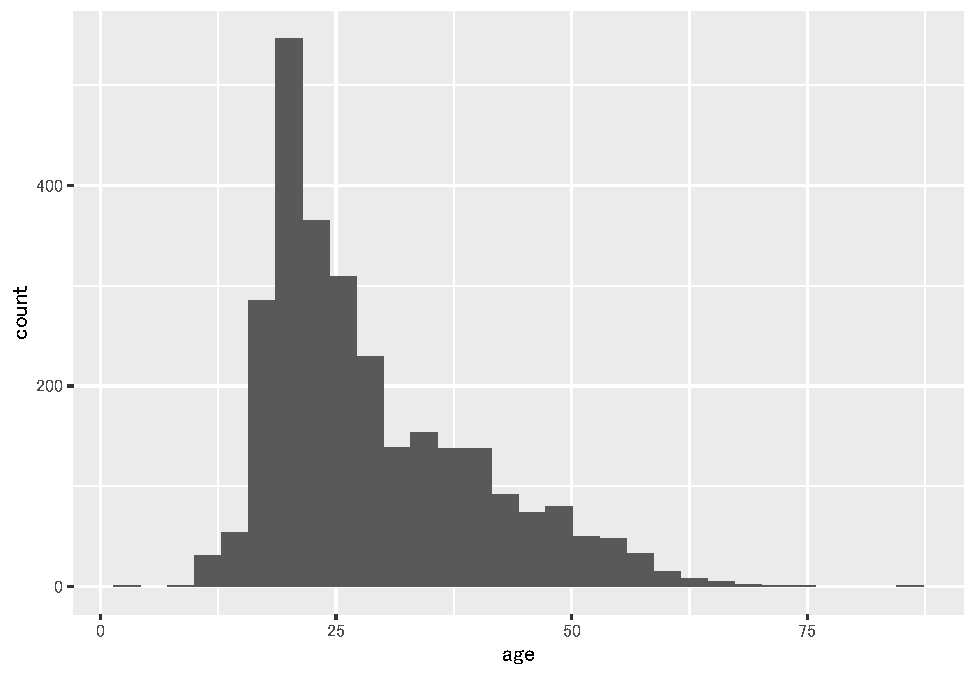
\includegraphics{gisho12_files/figure-latex/unnamed-chunk-79-1.pdf}

\begin{itemize}
\tightlist
\item
  さっと中央値だけ見たいのであれば,従来のRの書き方が早い
\item
  役に立つ場面が多いので,慣れたら従来の書き方を学んでおくとよい

  \begin{itemize}
  \tightlist
  \item
  \end{itemize}
\item
  \texttt{データフレーム\$変数名}と指定することで変数として扱える
\end{itemize}

\begin{Shaded}
\begin{Highlighting}[]
\CommentTok{\# 中央値}
\FunctionTok{median}\NormalTok{(df\_bfi}\SpecialCharTok{$}\NormalTok{age)}
\end{Highlighting}
\end{Shaded}

\begin{verbatim}
## [1] 26
\end{verbatim}

\begin{Shaded}
\begin{Highlighting}[]
\CommentTok{\# モダンな方法だと少し長くなる}
\CommentTok{\# df\_bfi \%\textgreater{}\% }
\CommentTok{\#   summarise(median(age))}
\end{Highlighting}
\end{Shaded}

\hypertarget{ux533aux5206}{%
\subsection{2区分}\label{ux533aux5206}}

\begin{itemize}
\tightlist
\item
  \texttt{dplyr::if\_else(\ )}で条件式(TRUEまたはFALSEを返すもの)によって値を2区分する
\item
  構造:\texttt{if\_else(条件式,\ TRUEの場合の値,\ FALSEの場合の値)}

  \begin{itemize}
  \tightlist
  \item
    TRUEの場合の値, FALSEの場合の値はそれぞれ文字型を入れることもできる(例:``27歳以上'', ``27歳未満'')
  \end{itemize}
\end{itemize}

\begin{Shaded}
\begin{Highlighting}[]
\NormalTok{res\_age2 }\OtherTok{\textless{}{-}} 
\NormalTok{  df\_bfi }\SpecialCharTok{\%\textgreater{}\%} 
  \FunctionTok{mutate}\NormalTok{(}\AttributeTok{age2 =} \FunctionTok{if\_else}\NormalTok{(age }\SpecialCharTok{\textgreater{}=} \DecValTok{27}\NormalTok{, }\DecValTok{1}\NormalTok{, }\DecValTok{0}\NormalTok{)) }\SpecialCharTok{\%\textgreater{}\%} 
  \FunctionTok{select}\NormalTok{(age, age2)}

\NormalTok{res\_age2 }\SpecialCharTok{\%\textgreater{}\%} \FunctionTok{count}\NormalTok{(age2) }
\end{Highlighting}
\end{Shaded}

\begin{verbatim}
## # A tibble: 2 x 2
##    age2     n
##   <dbl> <int>
## 1     0  1495
## 2     1  1305
\end{verbatim}

\hypertarget{ux78baux8a8d-1}{%
\subsubsection{確認}\label{ux78baux8a8d-1}}

\begin{itemize}
\tightlist
\item
  \texttt{age\ \textgreater{}=\ 27}が1,27未満が0にコーディングされているか\texttt{filter(\ )}で限定して確認
\end{itemize}

\begin{Shaded}
\begin{Highlighting}[]
\NormalTok{res\_age2 }\SpecialCharTok{\%\textgreater{}\%} 
  \FunctionTok{filter}\NormalTok{(age }\SpecialCharTok{\textgreater{}=} \DecValTok{20} \SpecialCharTok{\&}\NormalTok{ age }\SpecialCharTok{\textless{}=} \DecValTok{30}\NormalTok{) }\SpecialCharTok{\%\textgreater{}\%} 
  \FunctionTok{count}\NormalTok{(age, age2) }\SpecialCharTok{\%\textgreater{}\%} 
  \FunctionTok{print}\NormalTok{(}\AttributeTok{n =} \DecValTok{11}\NormalTok{)}
\end{Highlighting}
\end{Shaded}

\begin{verbatim}
## # A tibble: 11 x 3
##      age  age2     n
##    <int> <dbl> <int>
##  1    20     0   212
##  2    21     0   144
##  3    22     0   122
##  4    23     0   138
##  5    24     0   105
##  6    25     0   113
##  7    26     0    99
##  8    27     1    97
##  9    28     1    86
## 10    29     1    78
## 11    30     1    65
\end{verbatim}

\begin{itemize}
\tightlist
\item
  念のため最初3行(1-3行目)と最後3行(n-2行目からn行目)も確認
\item
  \texttt{dplyr::slice(\ )}で1:3行目と最後の3行を表示させる
\end{itemize}

\begin{Shaded}
\begin{Highlighting}[]
\NormalTok{res\_age2 }\SpecialCharTok{\%\textgreater{}\%} 
  \FunctionTok{count}\NormalTok{(age, age2) }\SpecialCharTok{\%\textgreater{}\%} 
  \FunctionTok{slice}\NormalTok{(}\DecValTok{1}\SpecialCharTok{:}\DecValTok{3}\NormalTok{, (}\FunctionTok{n}\NormalTok{()}\SpecialCharTok{{-}}\DecValTok{2}\NormalTok{)}\SpecialCharTok{:}\FunctionTok{n}\NormalTok{())}
\end{Highlighting}
\end{Shaded}

\begin{verbatim}
## # A tibble: 6 x 3
##     age  age2     n
##   <int> <dbl> <int>
## 1     3     0     1
## 2     9     0     1
## 3    11     0     3
## 4    72     1     1
## 5    74     1     1
## 6    86     1     1
\end{verbatim}

\begin{Shaded}
\begin{Highlighting}[]
\FunctionTok{rm}\NormalTok{(res\_age2)}
\end{Highlighting}
\end{Shaded}

\hypertarget{ux533aux5206ux4ee5ux4e0a}{%
\subsection{3区分以上}\label{ux533aux5206ux4ee5ux4e0a}}

\begin{itemize}
\tightlist
\item
  年齢層を10歳区切りでカテゴリ化
\end{itemize}

\begin{Shaded}
\begin{Highlighting}[]
\NormalTok{res\_age6 }\OtherTok{\textless{}{-}} 
\NormalTok{  df\_bfi }\SpecialCharTok{\%\textgreater{}\%} 
  \FunctionTok{mutate}\NormalTok{(}\AttributeTok{age6 =} \FunctionTok{case\_when}\NormalTok{(}
\NormalTok{    age }\SpecialCharTok{\textless{}} \DecValTok{20}              \SpecialCharTok{\textasciitilde{}} \StringTok{"20歳未満"}\NormalTok{, }
\NormalTok{    age }\SpecialCharTok{\textgreater{}=} \DecValTok{20}  \SpecialCharTok{\&}\NormalTok{ age }\SpecialCharTok{\textless{}} \DecValTok{30} \SpecialCharTok{\textasciitilde{}} \StringTok{"20{-}29歳"}\NormalTok{, }
\NormalTok{    age }\SpecialCharTok{\textgreater{}=} \DecValTok{30}  \SpecialCharTok{\&}\NormalTok{ age }\SpecialCharTok{\textless{}} \DecValTok{40} \SpecialCharTok{\textasciitilde{}} \StringTok{"30{-}39歳"}\NormalTok{,}
\NormalTok{    age }\SpecialCharTok{\textgreater{}=} \DecValTok{40}  \SpecialCharTok{\&}\NormalTok{ age }\SpecialCharTok{\textless{}} \DecValTok{50} \SpecialCharTok{\textasciitilde{}} \StringTok{"40{-}49歳"}\NormalTok{,}
\NormalTok{    age }\SpecialCharTok{\textgreater{}=} \DecValTok{50}  \SpecialCharTok{\&}\NormalTok{ age }\SpecialCharTok{\textless{}} \DecValTok{60} \SpecialCharTok{\textasciitilde{}} \StringTok{"50{-}59歳"}\NormalTok{,}
\NormalTok{    age }\SpecialCharTok{\textgreater{}=} \DecValTok{60}             \SpecialCharTok{\textasciitilde{}} \StringTok{"60歳以上"}  
\NormalTok{  ))}

\CommentTok{\# 確認するには以下のコードの最初の2行だけでよいが,出力が長いためランダムに10件抽出しageの昇順にしてある}
\NormalTok{res\_age6 }\SpecialCharTok{\%\textgreater{}\%} 
  \FunctionTok{count}\NormalTok{(age, age6) }\SpecialCharTok{\%\textgreater{}\%} 
  \FunctionTok{slice\_sample}\NormalTok{(}\AttributeTok{n =} \DecValTok{10}\NormalTok{) }\SpecialCharTok{\%\textgreater{}\%} \CommentTok{\# ランダムに10件抽出}
  \FunctionTok{arrange}\NormalTok{(age)             }\CommentTok{\# ageをキーに行を昇順にソート}
\end{Highlighting}
\end{Shaded}

\begin{verbatim}
## # A tibble: 10 x 3
##      age age6         n
##    <int> <chr>    <int>
##  1    19 20歳未満   190
##  2    23 20-29歳    138
##  3    26 20-29歳     99
##  4    28 20-29歳     86
##  5    31 30-39歳     73
##  6    38 30-39歳     52
##  7    61 60歳以上     4
##  8    62 60歳以上     4
##  9    65 60歳以上     1
## 10    70 60歳以上     1
\end{verbatim}

\begin{Shaded}
\begin{Highlighting}[]
\FunctionTok{rm}\NormalTok{(res\_age6)}
\end{Highlighting}
\end{Shaded}

\hypertarget{summarise}{%
\chapter{要約値を作る:summarise}\label{summarise}}

\begin{itemize}
\tightlist
\item
  パッケージ\texttt{dplyr}の関数\texttt{summarise()}
\item
  結果をデータフレームとして出力するため,扱いが便利
\item
  データを知るうえで要約作業は頻繁に行うことが想定される

  \begin{itemize}
  \tightlist
  \item
    便利な要約パッケージが色々あるものの,\texttt{summarise()}を使いこなせると役に立つことが多い
  \end{itemize}
\end{itemize}

\hypertarget{su-st}{%
\section{基本}\label{su-st}}

\begin{itemize}
\tightlist
\item
  \texttt{summarise(\ )}の中に出力したい変数名を書き,\texttt{=}の後に計算する関数を入れる
\item
  例:bill\_length\_mmの平均値を算出する
\end{itemize}

\begin{Shaded}
\begin{Highlighting}[]
\NormalTok{df }\SpecialCharTok{\%\textgreater{}\%} 
  \FunctionTok{summarise}\NormalTok{(blm\_平均値 }\OtherTok{=} \FunctionTok{mean}\NormalTok{(bill\_length\_mm, }\AttributeTok{na.rm =} \ConstantTok{TRUE}\NormalTok{))}
\end{Highlighting}
\end{Shaded}

\begin{verbatim}
## # A tibble: 1 x 1
##   blm_平均値
##        <dbl>
## 1       43.9
\end{verbatim}

\hypertarget{su-st-multiple}{%
\section{複数の計算}\label{su-st-multiple}}

\begin{itemize}
\tightlist
\item
  複数の変数について平均値とSDとnを出したいときは,基本知識では全部書くので長くなる
\end{itemize}

\begin{Shaded}
\begin{Highlighting}[]
\NormalTok{df }\SpecialCharTok{\%\textgreater{}\%} 
  \FunctionTok{summarise}\NormalTok{(}\AttributeTok{blm\_mean =} \FunctionTok{mean}\NormalTok{(bill\_length\_mm, }\AttributeTok{na.rm =} \ConstantTok{TRUE}\NormalTok{),}
            \AttributeTok{bdm\_mean =} \FunctionTok{mean}\NormalTok{(bill\_depth\_mm, }\AttributeTok{na.rm =} \ConstantTok{TRUE}\NormalTok{),}
            \AttributeTok{blm\_sd =} \FunctionTok{sd}\NormalTok{(bill\_length\_mm, }\AttributeTok{na.rm =} \ConstantTok{TRUE}\NormalTok{),}
            \AttributeTok{bdm\_sd =} \FunctionTok{sd}\NormalTok{(bill\_depth\_mm, }\AttributeTok{na.rm =} \ConstantTok{TRUE}\NormalTok{),}
            \AttributeTok{blm\_n  =} \FunctionTok{sum}\NormalTok{(}\SpecialCharTok{!}\FunctionTok{is.na}\NormalTok{(bill\_length\_mm)),}
            \AttributeTok{bdm\_n  =} \FunctionTok{sum}\NormalTok{(}\SpecialCharTok{!}\FunctionTok{is.na}\NormalTok{(bill\_depth\_mm)))}
\end{Highlighting}
\end{Shaded}

\begin{verbatim}
## # A tibble: 1 x 6
##   blm_mean bdm_mean blm_sd bdm_sd blm_n bdm_n
##      <dbl>    <dbl>  <dbl>  <dbl> <int> <int>
## 1     43.9     17.2   5.46   1.97   342   342
\end{verbatim}

\hypertarget{su-st-ef}{%
\subsection{【効率化】}\label{su-st-ef}}

\begin{itemize}
\tightlist
\item
  \ref{mu-kata-across}で出てきた\texttt{across()}がここでも有用
\item
  \texttt{across()}の第一引数に指定したい変数名ベクトル,またはヘルパー関数を入れる
\item
  実行したい関数をlist内に名前(接尾辞)をつけて列挙し,関数の前に\texttt{\textasciitilde{}}をつける
\item
  \texttt{sum(!is.na(.x))}は,NAのない行の数を総計するので,平均値やSDの計算に用いた人数を取得できる
\end{itemize}

\begin{Shaded}
\begin{Highlighting}[]
\NormalTok{df }\SpecialCharTok{\%\textgreater{}\%} 
  \FunctionTok{summarise}\NormalTok{(}\FunctionTok{across}\NormalTok{(}\FunctionTok{c}\NormalTok{(bill\_length\_mm, bill\_depth\_mm),}
                   \FunctionTok{list}\NormalTok{(}\AttributeTok{mean =} \SpecialCharTok{\textasciitilde{}}\FunctionTok{mean}\NormalTok{(.x, }\AttributeTok{na.rm =} \ConstantTok{TRUE}\NormalTok{),}
                        \AttributeTok{sd =} \SpecialCharTok{\textasciitilde{}}\FunctionTok{sd}\NormalTok{(.x, }\AttributeTok{na.rm =} \ConstantTok{TRUE}\NormalTok{),}
                        \AttributeTok{n =} \SpecialCharTok{\textasciitilde{}}\FunctionTok{sum}\NormalTok{(}\SpecialCharTok{!}\FunctionTok{is.na}\NormalTok{(.x)))))}
\end{Highlighting}
\end{Shaded}

\begin{verbatim}
## # A tibble: 1 x 6
##   bill_length_mm_mean bill_length_mm_sd bill_length_mm_n
##                 <dbl>             <dbl>            <int>
## 1                43.9              5.46              342
## # ... with 3 more variables: bill_depth_mm_mean <dbl>,
## #   bill_depth_mm_sd <dbl>, bill_depth_mm_n <int>
\end{verbatim}

\begin{itemize}
\tightlist
\item
  \texttt{across()}ではヘルパー関数が使える
\end{itemize}

\begin{Shaded}
\begin{Highlighting}[]
\NormalTok{df }\SpecialCharTok{\%\textgreater{}\%} 
  \FunctionTok{summarise}\NormalTok{(}\FunctionTok{across}\NormalTok{(}\FunctionTok{starts\_with}\NormalTok{(}\StringTok{"bill"}\NormalTok{),}
                   \FunctionTok{list}\NormalTok{(}\AttributeTok{mean =} \SpecialCharTok{\textasciitilde{}}\FunctionTok{mean}\NormalTok{(.x, }\AttributeTok{na.rm =} \ConstantTok{TRUE}\NormalTok{),}
                        \AttributeTok{sd =} \SpecialCharTok{\textasciitilde{}}\FunctionTok{sd}\NormalTok{(.x, }\AttributeTok{na.rm =} \ConstantTok{TRUE}\NormalTok{),}
                        \AttributeTok{n =} \SpecialCharTok{\textasciitilde{}}\FunctionTok{sum}\NormalTok{(}\SpecialCharTok{!}\FunctionTok{is.na}\NormalTok{(.x)))))}
\end{Highlighting}
\end{Shaded}

\begin{verbatim}
## # A tibble: 1 x 6
##   bill_length_mm_mean bill_length_mm_sd bill_length_mm_n
##                 <dbl>             <dbl>            <int>
## 1                43.9              5.46              342
## # ... with 3 more variables: bill_depth_mm_mean <dbl>,
## #   bill_depth_mm_sd <dbl>, bill_depth_mm_n <int>
\end{verbatim}

\hypertarget{su-st-reorder}{%
\subsection{【並び替え】}\label{su-st-reorder}}

\begin{itemize}
\tightlist
\item
  上記の出力は横に長いため見にくい
\item
  \texttt{tidyr::pivot\_longer()}で,データフレームの行列入れ替えができる
\item
  引数を\texttt{names\_pattern}と\texttt{names\_to}を下記のように指定することで,変数の接尾辞を列名にできる
\item
  下記コードの\texttt{summarise(\ )}部分の構造は前のチャンクと変数名以外同じ
\end{itemize}

\begin{Shaded}
\begin{Highlighting}[]
\NormalTok{df }\SpecialCharTok{\%\textgreater{}\%} 
  \FunctionTok{summarise}\NormalTok{(}\FunctionTok{across}\NormalTok{(bill\_length\_mm}\SpecialCharTok{:}\NormalTok{body\_mass\_g,}
                   \FunctionTok{list}\NormalTok{(}\AttributeTok{mean =} \SpecialCharTok{\textasciitilde{}}\FunctionTok{mean}\NormalTok{(.x, }\AttributeTok{na.rm =} \ConstantTok{TRUE}\NormalTok{),}
                        \AttributeTok{sd =} \SpecialCharTok{\textasciitilde{}}\FunctionTok{sd}\NormalTok{(.x, }\AttributeTok{na.rm =} \ConstantTok{TRUE}\NormalTok{),}
                        \AttributeTok{n =} \SpecialCharTok{\textasciitilde{}}\FunctionTok{sum}\NormalTok{(}\SpecialCharTok{!}\FunctionTok{is.na}\NormalTok{(.x))))) }\SpecialCharTok{\%\textgreater{}\%} 
  \FunctionTok{pivot\_longer}\NormalTok{(}\FunctionTok{everything}\NormalTok{(),}
               \AttributeTok{names\_to =} \FunctionTok{c}\NormalTok{(}\StringTok{"items"}\NormalTok{, }\StringTok{".value"}\NormalTok{), }\CommentTok{\# ".value"の部分を列名に}
               \AttributeTok{names\_pattern =} \StringTok{"(.*)\_(.*)"}\NormalTok{)    }\CommentTok{\# 正規表現}
\end{Highlighting}
\end{Shaded}

\begin{verbatim}
## # A tibble: 4 x 4
##   items               mean     sd     n
##   <chr>              <dbl>  <dbl> <int>
## 1 bill_length_mm      43.9   5.46   342
## 2 bill_depth_mm       17.2   1.97   342
## 3 flipper_length_mm  201.   14.1    342
## 4 body_mass_g       4202.  802.     342
\end{verbatim}

\hypertarget{su-group}{%
\section{層別(グループ別)集計}\label{su-group}}

\begin{itemize}
\tightlist
\item
  \texttt{group\_by(\ )}にグループを表す変数を指定するとできる
\end{itemize}

\begin{Shaded}
\begin{Highlighting}[]
\NormalTok{df }\SpecialCharTok{\%\textgreater{}\%} 
  \FunctionTok{group\_by}\NormalTok{(species) }\SpecialCharTok{\%\textgreater{}\%} 
  \FunctionTok{summarise}\NormalTok{(}\FunctionTok{across}\NormalTok{(}\FunctionTok{c}\NormalTok{(bill\_length\_mm, bill\_depth\_mm),}
                   \FunctionTok{list}\NormalTok{(}\AttributeTok{mean =} \SpecialCharTok{\textasciitilde{}}\FunctionTok{mean}\NormalTok{(.x, }\AttributeTok{na.rm =} \ConstantTok{TRUE}\NormalTok{),}
                        \AttributeTok{sd =} \SpecialCharTok{\textasciitilde{}}\FunctionTok{sd}\NormalTok{(.x, }\AttributeTok{na.rm =} \ConstantTok{TRUE}\NormalTok{))))}
\end{Highlighting}
\end{Shaded}

\begin{verbatim}
## # A tibble: 3 x 5
##   species   bill_length_mm_mean bill_length_mm_~ bill_depth_mm_m~
##   <fct>                   <dbl>            <dbl>            <dbl>
## 1 Adelie                   38.8             2.66             18.3
## 2 Chinstrap                48.8             3.34             18.4
## 3 Gentoo                   47.5             3.08             15.0
## # ... with 1 more variable: bill_depth_mm_sd <dbl>
\end{verbatim}

\begin{itemize}
\tightlist
\item
  グループを重ねることも可能
\end{itemize}

\begin{Shaded}
\begin{Highlighting}[]
\NormalTok{df }\SpecialCharTok{\%\textgreater{}\%} 
  \FunctionTok{group\_by}\NormalTok{(species, sex) }\SpecialCharTok{\%\textgreater{}\%} 
  \FunctionTok{summarise}\NormalTok{(}\FunctionTok{across}\NormalTok{(}\FunctionTok{c}\NormalTok{(bill\_length\_mm, bill\_depth\_mm),}
                   \FunctionTok{list}\NormalTok{(}\AttributeTok{mean =} \SpecialCharTok{\textasciitilde{}}\FunctionTok{mean}\NormalTok{(.x, }\AttributeTok{na.rm =} \ConstantTok{TRUE}\NormalTok{),}
                        \AttributeTok{sd =} \SpecialCharTok{\textasciitilde{}}\FunctionTok{sd}\NormalTok{(.x, }\AttributeTok{na.rm =} \ConstantTok{TRUE}\NormalTok{))))}
\end{Highlighting}
\end{Shaded}

\begin{verbatim}
## # A tibble: 8 x 6
## # Groups:   species [3]
##   species   sex    bill_length_mm_mean bill_length_mm_sd
##   <fct>     <fct>                <dbl>             <dbl>
## 1 Adelie    female                37.3              2.03
## 2 Adelie    male                  40.4              2.28
## 3 Adelie    <NA>                  37.8              2.80
## 4 Chinstrap female                46.6              3.11
## 5 Chinstrap male                  51.1              1.56
## 6 Gentoo    female                45.6              2.05
## 7 Gentoo    male                  49.5              2.72
## 8 Gentoo    <NA>                  45.6              1.37
## # ... with 2 more variables: bill_depth_mm_mean <dbl>,
## #   bill_depth_mm_sd <dbl>
\end{verbatim}

\hypertarget{su-fun}{%
\section{【効率化】関数にする}\label{su-fun}}

\hypertarget{su-fun-st}{%
\subsection{基本}\label{su-fun-st}}

\begin{itemize}
\tightlist
\item
  \texttt{自分で名づける関数名\ \textless{}-\ function(引数)\{\ 計算式やコード\ \}} で関数を定義できる
\item
  例:関数の引数に数値を入れると\texttt{+1}した値を返す関数
\end{itemize}

\begin{Shaded}
\begin{Highlighting}[]
\NormalTok{add\_one }\OtherTok{\textless{}{-}} 
  \ControlFlowTok{function}\NormalTok{(x)\{}
\NormalTok{    x }\SpecialCharTok{+} \DecValTok{1}
\NormalTok{  \}}

\FunctionTok{add\_one}\NormalTok{(}\DecValTok{2}\NormalTok{)}
\end{Highlighting}
\end{Shaded}

\begin{verbatim}
## [1] 3
\end{verbatim}

\hypertarget{su-fun-meansdn}{%
\subsection{複数変数の平均値とSDとnを計算する関数}\label{su-fun-meansdn}}

\begin{itemize}
\tightlist
\item
  \texttt{\{\{\ \}\}}は\texttt{curly\ curly}と読み,関数を作成するときに,代入先の変数名の場所を指定する時などに活躍

  \begin{itemize}
  \tightlist
  \item
    下記の例の場合,\texttt{\{\{\ \}\}}を外すと動かない
  \end{itemize}
\item
  例:引数にデータフレーム(data)と変数(vars)を入れると平均値とSDとnを返す関数
\end{itemize}

\begin{Shaded}
\begin{Highlighting}[]
\NormalTok{mean\_sd\_n }\OtherTok{\textless{}{-}} \ControlFlowTok{function}\NormalTok{(data, vars)\{}
\NormalTok{data }\SpecialCharTok{\%\textgreater{}\%} 
  \FunctionTok{summarise}\NormalTok{(}\FunctionTok{across}\NormalTok{(\{\{vars\}\},}
                   \FunctionTok{list}\NormalTok{(}\AttributeTok{mean =} \SpecialCharTok{\textasciitilde{}}\FunctionTok{mean}\NormalTok{(.x, }\AttributeTok{na.rm =} \ConstantTok{TRUE}\NormalTok{),}
                        \AttributeTok{sd =} \SpecialCharTok{\textasciitilde{}}\FunctionTok{sd}\NormalTok{(.x, }\AttributeTok{na.rm =} \ConstantTok{TRUE}\NormalTok{),}
                        \AttributeTok{n =} \SpecialCharTok{\textasciitilde{}}\FunctionTok{sum}\NormalTok{(}\SpecialCharTok{!}\FunctionTok{is.na}\NormalTok{(.x)))))}
\NormalTok{\}}
\end{Highlighting}
\end{Shaded}

\begin{itemize}
\tightlist
\item
  ここで定義した関数\texttt{mean\_sd\_n(\ )}にデータフレームと変数を入れると結果が表示される
\end{itemize}

\begin{Shaded}
\begin{Highlighting}[]
\FunctionTok{mean\_sd\_n}\NormalTok{(df, bill\_length\_mm)}
\end{Highlighting}
\end{Shaded}

\begin{verbatim}
## # A tibble: 1 x 3
##   bill_length_mm_mean bill_length_mm_sd bill_length_mm_n
##                 <dbl>             <dbl>            <int>
## 1                43.9              5.46              342
\end{verbatim}

\begin{itemize}
\tightlist
\item
  vasの部分は\texttt{across(\ )}の第一引数に入れるものと同じ指定ができるため,変数ベクトルやヘルパー関数が入る
\end{itemize}

\begin{Shaded}
\begin{Highlighting}[]
\CommentTok{\# 変数ベクトル}
\FunctionTok{mean\_sd\_n}\NormalTok{(df, }\FunctionTok{c}\NormalTok{(flipper\_length\_mm, body\_mass\_g))}
\end{Highlighting}
\end{Shaded}

\begin{verbatim}
## # A tibble: 1 x 6
##   flipper_length_mm_mean flipper_length_mm_sd flipper_length_mm_n
##                    <dbl>                <dbl>               <int>
## 1                   201.                 14.1                 342
## # ... with 3 more variables: body_mass_g_mean <dbl>,
## #   body_mass_g_sd <dbl>, body_mass_g_n <int>
\end{verbatim}

\begin{Shaded}
\begin{Highlighting}[]
\CommentTok{\# 文字でも可能}
\CommentTok{\# mean\_sd\_n(df, c("flipper\_length\_mm", "body\_mass\_g"))}

\CommentTok{\# ヘルパー関数}
\FunctionTok{mean\_sd\_n}\NormalTok{(df, }\FunctionTok{starts\_with}\NormalTok{(}\StringTok{"bill"}\NormalTok{))}
\end{Highlighting}
\end{Shaded}

\begin{verbatim}
## # A tibble: 1 x 6
##   bill_length_mm_mean bill_length_mm_sd bill_length_mm_n
##                 <dbl>             <dbl>            <int>
## 1                43.9              5.46              342
## # ... with 3 more variables: bill_depth_mm_mean <dbl>,
## #   bill_depth_mm_sd <dbl>, bill_depth_mm_n <int>
\end{verbatim}

\hypertarget{ux3042ux3068ux304cux304d}{%
\chapter*{あとがき}\label{ux3042ux3068ux304cux304d}}
\addcontentsline{toc}{chapter}{あとがき}

あとがき

本書の執筆にあたり、同人誌制作の先輩である\texttt{天川榎@EnokiAmakawa}氏から背中押し&多くの助言をいただきました。この場を借りてお礼申し上げます。

\clearpage
\vspace*{\stretch{1}}
\begin{flushright}
\begin{minipage}{0.5\hsize}
\begin{description}
  \item{著者:} やわらかクジラ
  \item{発行:} 2020年9月12日
  \item{サークル名:} ヤサイゼリー
  \item{twitter:} @matsuchiy
  \item{印刷:} 電子出版のみ
\end{description}
\end{minipage}
\end{flushright}
\clearpage

\end{document}
